\chapter{Finding Alternative Feature Sets}
\label{sec:afs}

\section{Overview}
\label{sec:afs:overview}

\paragraph{Scope}

Our case study in Chapter~\ref{sec:ms} showed that differently composed feature sets of similar quality may exist.
However, these particular alternative feature sets were only a side-effect of employing different domain-specific constraints.
Nevertheless, obtaining such alternative solutions is generally desirable for users (cf.~Section~\ref{sec:introduction:research-gaps:finding-alternative-solutions}).
In this chapter, we formally introduce alternative feature selection in a domain-independent manner.
This new problem definition instantiates constrained feature selection (cf.~Chapter~\ref{sec:syn}) with particular constraint types.
Users can employ these predefined constraint types and configure them with user-friendly parameters.

\paragraph{Contributions}

Our contribution in this chapter is fivefold.

(1) We formalize alternative feature selection as an optimization problem, using 0-1 integer linear constraints to express alternative feature sets.
This approach is orthogonal to the feature-selection method so that users can choose the latter according to their needs.
Additionally, users may add further constraints on feature sets, e.g., to capture domain knowledge.
We let users control the search for alternatives with two parameters, i.e., the number of alternatives and a dissimilarity threshold.
For multiple alternatives, we consider sequential and simultaneous search.

(2) We discuss how to solve this optimization problem.
To that end, we describe how to integrate different categories of conventional feature-selection methods into the optimization problem's objective function.
In particular, we outline solver-based search methods for white-box and black-box optimization.

(3) We analyze the time complexity of the problem.
We show $\mathcal{NP}$-hardness, even for a simple notion of feature-set quality, i.e., univariate feature qualities.

(4) We propose heuristic search methods for univariate feature qualities.
We show that, under certain conditions, the optimization problem resides in the complexity class $\mathcal{APX}$, i.e., a constant-factor approximation exists.

(5) We conduct comprehensive experiments with 30 binary-classification datasets from the Penn Machine Learning Benchmarks (PMLB)~\cite{olson2017pmlb, romano2021pmlb} and five feature-selection methods.
We evaluate feature-set quality and runtime to investigate our search methods for alternatives and their user parameters.
Section~\ref{sec:afs:evaluation:summary} summarizes key results.

\paragraph{Materials}

We publish all our code and experimental data online (cf.~Section~\ref{sec:introduction:materials}).

\paragraph{Prior works}

The content of this chapter bases on the following prior works:
%
\begin{itemize}
	\item \fullcite{bach2023finding}
	\item \fullcite{bach2024alternative}
\end{itemize}

\paragraph{Chapter outline}

The remainder of this chapter is structured as follows:
Section~\ref{sec:afs:approach} describes and analyzes alternative feature selection.
Section~\ref{sec:afs:experimental-design} outlines our experimental design.
Section~\ref{sec:afs:evaluation} presents the corresponding experimental results.

\section{Alternative Feature Selection}
\label{sec:afs:approach}

In this section, we present the problem and approaches for alternative feature selection.
First, we define the overall structure of the optimization problem (cf.~Section~\ref{sec:afs:approach:problem}).
Second, we formalize alternatives via constraints (cf.~Section~\ref{sec:afs:approach:constraints}).
Third, we discuss objective functions for different feature-set quality measures and describe how to solve the resulting optimization problem (cf.~Section~\ref{sec:afs:approach:objectives}).
Fourth, we analyze the problem's time complexity (cf.~Section~\ref{sec:afs:approach:complexity}).
Fifth, we propose and analyze heuristic search methods for univariate feature qualities in the objective (cf.~Section~\ref{sec:afs:approach:univariate-heuristics}).

\subsection{Optimization Problem}
\label{sec:afs:approach:problem}

Alternative feature selection has two goals.
First, the quality of an alternative feature set should be high, as in conventional feature selection (cf.~Definition~\ref{def:fs:feature-selection}).
Second, an alternative feature set should differ from one or more other feature set(s).
There are several ways to combine these two goals in an optimization problem:

First, one can consider both goals as objectives, obtaining an unconstrained multi-objective problem.
Second, one can define constraints for both, feature-set quality and being alternative, searching for feasible solutions instead of optimizing.
Third, one can consider being alternative as objective and constrain feature-set quality, e.g., with a lower bound.
Fourth, one can treat feature-set quality as objective and enforce alternatives with constraints.

We pursue the last formulation, i.e., optimizing feature-set quality subject to being alternative.
This formulation is a special case of constrained feature selection (cf.~Definition~\ref{def:syn:constrained-feature-selection}) and keeps the original objective of feature selection.
Users need not set a threshold on feature-set quality but control how alternative the feature sets must be instead.
We obtain the following optimization problem for a single alternative feature set~$F_s$:

\begin{equation}
	\begin{aligned}
		\max_s &\quad Q(s,X,y) \\
		\text{subject to:} &\quad F_s~\text{being alternative}
	\end{aligned}
	\label{eq:afs:afs-general}
\end{equation}
%
In the following, we discuss different objective functions $Q(s,X,y)$ (cf.~Section~\ref{sec:afs:approach:objectives}) and suitable constraints for feature sets \emph{being alternative} (cf.~Section~\ref{sec:afs:approach:constraints}).
As in the previous chapter, we also typically limit the feature-set size $|F_s|$ to a user-defined value~$k \in \mathbb{N}$, which adds a further, simple constraint (cf.~Equation~\ref{eq:syn:cardinality}) to the optimization problem.

\subsection{Constraints -- Defining Alternatives}
\label{sec:afs:approach:constraints}

In this section, we formalize alternative feature sets.
First, we discuss the base case where an individual feature set is an alternative to another one (cf.~Section~\ref{sec:afs:approach:constraints:single}).
Second, we extend this notion to multiple alternatives, considering sequential and simultaneous search as two different problems (cf.~Section~\ref{sec:afs:approach:constraints:multiple}).
Our notion of alternatives is independent of the feature-selection method.
We provide two parameters, i.e., a dissimilarity threshold~$\tau$ and the number of alternatives~$a$, allowing users to control the search for alternatives.

\subsubsection{Single Alternative}
\label{sec:afs:approach:constraints:single}

We consider a feature set an alternative to another if it differs sufficiently.
Formally, we express this notion with a set-dissimilarity measure~\cite{choi2010survey, egghe2009new}.
Such measures typically assess set overlap and set sizes.
E.g., a well-known set-dissimilarity measure is the Jaccard distance, which is defined as follows for the (feature) sets $F'$ and $F''$:
%
\begin{equation}
	d_{\text{Jacc}}(F',F'') = 1 - \frac{|F' \cap F''|}{|F' \cup F''|} = 1 - \frac{|F' \cap F''|}{|F'| + |F''| - |F' \cap F''|}
	\label{eq:afs:jaccard}
\end{equation}
%
In this dissertation, we use a dissimilarity measure based on the Dice coefficient:
%
\begin{equation}
	d_{\text{Dice}}(F',F'') = 1 - \frac{2 \cdot |F' \cap F''|}{|F'| + |F''|}
	\label{eq:afs:dice}
\end{equation}
%
Generally, we only have mild assumptions on the set-dissimilarity measure~$d(\cdot)$.
Our subsequent definitions, examples, and propositions assume symmetry, i.e., $d(F',F'')=d(F'',F')$, normalization $d(\cdot) \in [0,1]$, and that $d(\cdot) = 1$ implies an empty intersection of the two sets.
In particular, $d(\cdot)$~does not need to be a metric but can also be a semi-metric~\cite{wilson1931semi} like~$d_{\text{Dice}}(\cdot)$.
In contrast to metrics, semi-metrics may violate the triangle inequality.

We leverage the set-dissimilarity measure~$d(\cdot)$ for the following definition:
%
\begin{definition}[Single alternative]
	Given a symmetric set-dissimilarity measure~$d(\cdot) \in [0, 1]$ with $d(\cdot) = 1$ implying no set overlap, and a dissimilarity threshold~$\tau \in [0, 1]$, a feature set $F'$ is an alternative to a feature set~$F''$ (and vice versa) if $d(F',F'') \geq \tau$.
	\label{def:afs:single-alternative}
\end{definition}
%
The threshold~$\tau$ controls how dissimilar alternative feature sets must be.
A larger~$\tau$ may reduce feature-set quality more, but the exact impact depends on the dataset and is unclear a priori.
Also, only users can decide which drop in feature-set quality is acceptable as a trade-off for obtaining alternatives.
Thus, we leave $\tau$ as a user parameter.
For dissimilarity measures $d(\cdot)$ with range $[0,1]$, like the Dice dissimilarity (cf.~Equation~\ref{eq:afs:dice}) or Jaccard distance (cf.~Equation~\ref{eq:afs:jaccard}), $\tau$~has a user-friendly interpretation:
$\tau=0$ allows identical feature sets, while $\tau=1$ implies zero overlap.
Users can adjust~$\tau$ to find an acceptable quality-dissimilarity trade-off, e.g., with a binary search over $\tau$'s range.

When implementing Definition~\ref{def:afs:single-alternative}, the following proposition gives way to using a broad range of solvers to tackle the related optimization problem:
%
\begin{proposition}[Linearity of constraints for alternatives]
	Using the Dice dissimilarity (cf.~Equation~\ref{eq:afs:dice}), alternative feature sets (cf.~Definition~\ref{def:afs:single-alternative}) can be expressed with 0-1 integer linear constraints.
	\label{prop:afs:linear-constraints}
\end{proposition}
%
\begin{proof}
	We re-arrange terms in the Dice dissimilarity (cf.~Equation~\ref{eq:afs:dice}) to eliminate the quotient of feature-set sizes:
	%
	\begin{equation}
		\begin{aligned}
			d_{\text{Dice}}(F',F'') &= & 1 - \frac{2 \cdot |F' \cap F''|}{|F'| + |F''|} &\geq \tau \\
			&\Leftrightarrow & |F' \cap F''| &\leq \frac{1 - \tau}{2} \cdot (|F'| + |F''|)
		\end{aligned}
		\label{eq:afs:dice-rearranged}
	\end{equation}
	%
	Next, we express the set sizes in terms of the feature-selection vector $s$:
	%
	\begin{equation}
		\begin{aligned}
			|F_s| =& \sum_{j=1}^n s_j \\
			|F_{s'} \cap F_{s''}| =& \sum_{j=1}^n s'_j \cdot s''_j
		\end{aligned}
		\label{eq:afs:feature-set-size}
	\end{equation}
	%
	Finally, we replace each product $s'_j \cdot s''_j$ with an auxiliary variable~$t_j$, bound by additional constraints, to linearize it~\cite{mosek2022modeling}:
	%
	\begin{equation}
		\begin{aligned}
			t_j \leq& s'_j \\
			t_j \leq& s''_j \\
			1 + t_j \geq& s'_j + s''_j \\
			t_j \in& \{0,1\}
		\end{aligned}
		\label{eq:afs:product-linear}
	\end{equation}
	%
	Combining Equations~\ref{eq:afs:dice-rearranged},~\ref{eq:afs:feature-set-size}, and~\ref{eq:afs:product-linear}, we obtain a set of constraints that only involve linear expressions of binary decision variables.
	In particular, there are only sum expressions and multiplications with constants but no products between variables.
	If one feature set is known, i.e., either $s'$ or $s''$ is fixed, Equation~\ref{eq:afs:feature-set-size} is already linear without Equation~\ref{eq:afs:product-linear}.
\end{proof}
%
Given a suitable objective function, which we discuss in Section~\ref{sec:afs:approach:objectives}, linear constraints allow using a broad range of solvers.
Alternatively, one could also encode these constraints into propositional logic (SAT)~\cite{ulrich2022selecting} to enable using another category of solvers.

If the set sizes $|F'|$ and $|F''|$ are constant, e.g., a user-defined~$k \in \mathbb{N}$, Equation~\ref{eq:afs:dice-rearranged} implies that the threshold~$\tau$ has a linear relationship to the maximum number of overlapping features~$|F' \cap F''|$.
This correspondence makes~$\tau$ easy to interpret, so we use the Dice dissimilarity in the following.
In contrast, the Jaccard distance leads to a non-linear relationship between $\tau$ and the overlap size (cf.~Definition~\ref{def:afs:single-alternative} with Equation~\ref{eq:afs:jaccard}):
%
\begin{equation}
	\begin{aligned}
		d_{\text{Jacc}}(F',F'') &= & 1 - \frac{|F' \cap F''|}{|F'| + |F''| - |F' \cap F''|} &\geq \tau \\
		&\Leftrightarrow & |F' \cap F''| &\leq \frac{1 - \tau}{2 - \tau} \cdot (|F'| + |F''|)
	\end{aligned}
	\label{eq:afs:jaccard-rearranged}
\end{equation}
%
Further, if $|F'| = |F''|$, as in our experiments, the Dice dissimilarity becomes identical to several other set-dissimilarity measures~\cite{egghe2009new}.
The parameter~$\tau$ then directly expresses which fraction of features in one set needs to differ from the other set and vice versa:
%
\begin{equation}
	d_{\text{Dice}}(F',F'') \geq \tau \Leftrightarrow |F' \cap F''| \leq (1 - \tau) \cdot |F'| = (1 - \tau) \cdot |F''|
	\label{eq:afs:dice-rearranged-equal-size}
\end{equation}
%
Thus, if users are uncertain how to choose $\tau$ and $|F'|$ is reasonably small, they can try out all values of $\tau \in \{l / |F'|\}$ with $l \in \{1, \dots, |F'|\}$.
In particular, these $|F'|$~unique values of $\tau$ suffice to produce all distinct solutions that one could obtain with an arbitrary $\tau \in (0,1]$.

\subsubsection{Multiple Alternatives}
\label{sec:afs:approach:constraints:multiple}

If users desire multiple alternative feature sets rather than only one, we can determine these alternatives sequentially or simultaneously.
The number of alternatives~$a \in \mathbb{N}_0$ is a parameter to be set by the user.
The overall number of feature sets is $a + 1$ since we deem one feature set the \emph{original} one.
Table~\ref{tab:afs:seq-sim-comparison} shows the sizes of the two search problems.

\begin{table}[t]
	\centering
	\caption{Number of variables and constraints for $a$~alternatives ($a + 1$~feature sets overall) and $n$ features.}
	\renewcommand*{\arraystretch}{1.3}
	\begin{tabular}{lccc}
		\toprule
		& \multicolumn{2}{c}{Sequential search} & \multirow{2}{*}{Simultaneous search} \\
		\cmidrule(lr){2-3}
		& $l$-th Alternative & Summed & \\
		\midrule
		Decision variables~$s$ & $n$ & $ (a+1) \cdot n$ & $(a+1) \cdot n$ \\
		Linearization variables~$t$ & $0$ & $0$ & $\frac{a \cdot (a+1) \cdot n}{2}$ \\
		Alternative constraints & $l$ & $\frac{a \cdot (a+1)}{2}$ & $\frac{a \cdot (a+1)}{2}$ \\
		Linearization constraints & $0$ & $0$ & $\frac{3 \cdot a \cdot (a+1) \cdot n}{2}$ \\
		\bottomrule
	\end{tabular}
	\label{tab:afs:seq-sim-comparison}
\end{table}

\paragraph{Sequential-search problem}

In the sequential-search problem, users obtain several alternatives iteratively, with one feature set per iteration.
We constrain this new set to be an alternative to all previously found ones, which are given in a set~$\mathbb{F}$:
%
\begin{definition}[Sequential alternative]
	A feature set~$F''$ is an alternative to a set of feature sets~$\mathbb{F}$ (and vice versa) if $F''$ is a single alternative (cf.~Definition~\ref{def:afs:single-alternative}) to each $F' \in \mathbb{F}$.
	\label{def:afs:sequential-alternative}
\end{definition}
%
One could also think of less strict constraints, e.g., only bounding the average dissimilarity to all previously found feature sets.
However, definitions like the latter may allow some feature sets to overlap heavily or even be identical if others are very dissimilar.
Thus, we require pairwise dissimilarity in Definition~\ref{def:afs:sequential-alternative}.
Combining Equation~\ref{eq:afs:afs-general} with Definition~\ref{def:afs:sequential-alternative}, we obtain the following optimization problem for each iteration of the search:
%
\begin{equation}
	\begin{aligned}
		\max_s &\quad Q(s,X,y) \\
		\text{subject to:} &\quad \forall F' \in \mathbb{F}:~d(F_s,F') \geq \tau
	\end{aligned}
	\label{eq:afs:afs-sequential}
\end{equation}
%
The full textual problem definition corresponding to Equation~\ref{eq:afs:afs-sequential} is the following:
%
\begin{definition}[Sequential-search problem for one alternative feature set]
	Given
	\begin{itemize}[noitemsep]
		\item a dataset~$X \in \mathbb{R}^{m \times n}$ with prediction target~$y \in Y^m$,
		\item a set~$\mathbb{F}$ of existing feature sets for~$X$,
		\item a symmetric set-dissimilarity measure~$d(\cdot) \in [0,1]$ with $d(\cdot) = 1 \rightarrow$ no set overlap,
		\item and a dissimilarity threshold~$\tau \in [0,1]$,
	\end{itemize}
	sequential search for one alternative feature set is the problem of making feature-selection decisions~$s \in \{0,1\}^n$ that maximize a given notion of feature-set quality~$Q(s,X,y)$ while making the corresponding feature set~$F_s$ a sequential alternative to~$\mathbb{F}$ (cf.~Definition~\ref{def:afs:sequential-alternative}).
	\label{def:afs:alternative-feature-selection-sequential}
\end{definition}
%
We solve this optimization problem repeatedly, thereby optimizing only one feature set's quality at once.
$\mathbb{F} = \emptyset$ in the first iteration yields the \emph{original} feature set, i.e., the best unconstrained feature set.
Each alternative enlarges~$\mathbb{F}$ and adds one constraint, but the number of decision variables remains the same.
Further, we do not need to introduce linearization variables (cf.~Equation~\ref{eq:afs:product-linear}) since all feature sets except one are fixed.
Thus, the runtime of a solver-based sequential search should scale well with the number of alternatives.
Additional runtime gains may arise if the solver keeps a state between iterations and can warm-start.
Further, users do not need to define the number of alternatives a priori but can stop after each iteration once the feature-set quality is too low.
As a caveat, the stepwise optimization may yield alternatives with significantly different quality.

\paragraph{Simultaneous-search problem}

In the simultaneous-search problem, users obtain multiple alternatives at once, so they need to decide on the number of alternatives~$a$ beforehand.
We use pairwise dissimilarity constraints for alternatives again:
%
\begin{definition}[Simultaneous alternatives]
	A set of feature sets~$\mathbb{F}$ contains simultaneous alternatives if each feature set~$F' \in \mathbb{F}$ is a single alternative (cf.~Definition~\ref{def:afs:single-alternative}) to each other feature set~$F'' \in \mathbb{F}$ with $F' \neq F''$.
	\label{def:afs:simultaneous-alternative}
\end{definition}
%
Combining Equation~\ref{eq:afs:afs-general} with Definition~\ref{def:afs:simultaneous-alternative}, we obtain the following optimization problem for $a+1$ feature sets, i.e., including the original feature set:
%
\begin{equation}
	\begin{aligned}
		\max_{s^{(0)}, \dots, s^{(a)}} &\quad \operatorname*{agg}_{l \in \{0, \dots, a\}} Q(s^{(l)},X,y) \\
		\text{subject to:} &\quad \forall l_1, l_2 \in \{0, \dots, a\},~l_1 \neq l_2:~d(F_{s^{(l_1)}},F_{s^{(l_2)}}) \geq \tau
	\end{aligned}
	\label{eq:afs:afs-simultaneous}
\end{equation}
%
The full textual problem definition corresponding to Equation~\ref{eq:afs:afs-simultaneous} is the following:
%
\begin{definition}[Simultaneous-search problem for alternative feature sets]
	Given
	\begin{itemize}[noitemsep]
		\item a dataset~$X \in \mathbb{R}^{m \times n}$ with prediction target~$y \in Y^m$,
		\item the number of alternatives~$a \in \mathbb{N}_0$,
		\item an aggregation operator $\text{agg}(\cdot): \mathbb{R}^{a+1} \to \mathbb{R}$ for feature-set qualities,
		\item a symmetric set-dissimilarity measure~$d(\cdot) \in [0,1]$ with $d(\cdot) = 1 \rightarrow$ no set overlap,
		\item and a dissimilarity threshold~$\tau \in [0,1]$,
	\end{itemize}
	simultaneous search for alternative feature sets is the problem of making feature-selection decisions~$s^{(l)} \in \{0,1\}^n$ for $l \in \{0, \dots, a\}$ that maximize a given notion of feature-set quality~$Q(s,X,y)$ aggregated over the alternatives with $\operatorname*{agg}_{l \in \{0, \dots, a\}} Q(s^{(l)},X,y)$ while making the corresponding feature sets $\mathbb{F} = \{F_{s^{(0)}}, \dots, F_{s^{(a)}}\}$ simultaneous alternatives (cf.~Definition~\ref{def:afs:simultaneous-alternative}).
	\label{def:afs:alternative-feature-selection-simultaneous}
\end{definition}
%
In contrast to the sequential case (cf.~Definition~\ref{def:afs:alternative-feature-selection-sequential}), the problem requires $a+1$ instead of one decision vector~$s$ of length~$n$, and a modified objective function.
The operator~$\text{agg}(\cdot)$ defines how to aggregate the feature-set qualities of the alternatives, which we discuss later.
Runtime-wise, exact simultaneous search should scale worse with the number of alternatives than exact sequential search, as it tackles one large optimization problem instead of multiple smaller ones.
Besides requiring more decision variables, we need to introduce an auxiliary variable for each feature and pair of alternatives if we want to obtain linear constraints (cf.~Equation~\ref{eq:afs:product-linear} and Table~\ref{tab:afs:seq-sim-comparison}).
Quality-wise, simultaneous search may have an advantage over sequential search due to optimizing alternatives globally rather than greedily.
Also, the quality can be more evenly distributed over the alternatives, as opposed to the dropping quality over the course of the sequential procedure.
As a downside, there are no intermediate steps where users could interrupt the search.

\paragraph{Sum-aggregation}

One straightforward way to aggregate the qualities of feature sets in the simultaneous-search objective is to sum them up, which we call \emph{sum-aggregation}:
%
\begin{equation}
	\max_{s^{(0)}, \dots, s^{(a)}} \sum_{l=0}^a Q(s^{(l)},X,y)
	\label{eq:afs:afs-simultaneous-sum-objective}
\end{equation}
%
While this objective fosters a high average feature-set quality, it does not guarantee that the alternatives have similar quality:
%
\begin{example}[Sum-aggregation]
	Consider $n=6$~features with univariate feature qualities (cf.~Equation~\ref{eq:fs:univariate-filter}) $q = (9,8,7,3,2,1)$, feature-set size~$k=3$, number of alternatives~$a=2$, the Dice dissimilarity (cf.~Equation~\ref{eq:afs:dice}) as~$d(\cdot)$, and dissimilarity threshold~$\tau = 0.5$, which permits an overlap of one feature between sets here (cf.~Equation~\ref{eq:afs:dice-rearranged-equal-size}).
	Exact sequential search (cf.~Definition~\ref{def:afs:alternative-feature-selection-sequential}) yields the selection $s^{(0)} = (1,1,1,0,0,0)$, $s^{(1)} = (1,0,0,1,1,0)$, and $s^{(2)} = (0,1,0,1,0,1)$, with a summed quality of $\,24+14+12=50$.
	One possible exact simultaneous-search (cf.~Definition~\ref{def:afs:alternative-feature-selection-simultaneous}) solution consists of the feature sets $s^{(0)} = (1,1,0,1,0,0)$, $s^{(1)} = (1,0,1,0,1,0)$, and $s^{(2)} = (0,1,1,0,0,1)$, with a summed quality of $\,20+18+16=54$.
	Another possible exact simultaneous-search solution is $s^{(0)} = (1,1,0,0,0,1)$, $s^{(1)} = (1,0,1,0,1,0)$, and $s^{(2)} = (0,1,1,1,0,0)$, with a summed quality of $\,18+18+18=54$.
	\label{ex:afs:sum-aggregation}
\end{example}
%
This example yields several insights.
First, exact sequential search yields worse quality than exact simultaneous search here, i.e., 50 vs.~54.
Second, the feature-set qualities of the sequential solution, i.e., 24, 14, and~12, differ significantly.
Third, an exact simultaneous search can admit multiple solutions whose feature-set quality is differently balanced.
I.e., the solution with feature-set qualities 18, 18, and~18 is more balanced than the one with 20, 18, and~16.
However, both solutions are equally optimal for sum-aggregation.

\paragraph{Min-aggregation}

To actively foster balanced feature-set qualities in simultaneous search, we propose \emph{min-aggregation} in the objective:
%
\begin{equation}
	\max_{s^{(0)}, \dots, s^{(a)}} \min_{l \in \{0, \dots, a\}} Q(s^{(l)},X,y) \\
	\label{eq:afs:afs-simultaneous-min-objective}
\end{equation}
%
This formulation maximizes the quality of the worst alternative.
Thereby, it incentivizes all alternatives to have high quality and implicitly balances their quality.
In the terminology of social choice theory, it uses an egalitarian rule instead of a utilitarian one~\cite{myerson1981utilitarianism}.

Optimizing with either sum-aggregation or min-aggregation does not necessarily optimize the other.
Example~\ref{ex:afs:sum-aggregation} already showed a solution optimizing sum-aggregation but not min-aggregation.
In the following, we demonstrate the other direction:
%
\begin{example}[Min-aggregation]
	Consider $n=6$~features with univariate feature qualities (cf.~Equation~\ref{eq:fs:univariate-filter}) $q = (11,10,6,5,4,1)$, feature-set size~$k=3$, number of alternatives~$a=1$, the Dice dissimilarity (cf.~Equation~\ref{eq:afs:dice}) as~$d(\cdot)$, and dissimilarity threshold~$\tau = 0.5$, which permits an overlap of one feature between sets here (cf.~Equation~\ref{eq:afs:dice-rearranged-equal-size}).
	One simultaneous-search (cf.~Definition~\ref{def:afs:alternative-feature-selection-simultaneous}) solution with min-aggregation (cf.~Equation~\ref{eq:afs:afs-simultaneous-min-objective}) is $s^{(0)} = (1,1,0,0,1,0)$ and $s^{(1)} = (1,0,1,1,0,0)$, with a summed quality of $\,25+22=47$.
	Another solution is $s^{(0)} = (1,1,0,0,0,1)$ and $s^{(1)} = (1,0,1,1,0,0)$, with a summed quality of $\,22+22=44$.
	\label{ex:afs:min-aggregation}
\end{example}
%
While both solutions have the same minimum feature-set quality, only the first solution optimizes sum-aggregation.
In particular, min-aggregation permits reducing the quality of feature sets as long as the latter remains above the minimum quality of all sets.

From the technical perspective, Equation~\ref{eq:afs:afs-simultaneous-min-objective} has the disadvantage of being non-linear regarding the decision variables $s^{(0)}, \dots, s^{(a)}$.
However, we can linearize it with an auxiliary variable~$Q_{\text{min}}$ and one constraint per feature set:
%
\begin{equation}
	\begin{aligned}
		\max_{s^{(0)}, \dots, s^{(a)}} &\quad &Q_{\text{min}} & \\
		\text{subject to:} &\quad \forall l \in \{0, \dots, a\}: &Q_{\text{min}} &\leq Q(s^{(l)},X,y) \\
		&\quad & Q_{\text{min}} &\in \mathbb{R}
	\end{aligned}
	\label{eq:afs:afs-simultaneous-min-objective-linear}
\end{equation}
%
As we maximize~$Q_{\text{min}}$, this variable will implicitly assume the actual minimum value of~$Q(s^{(l)},X,y)$ with equality since the solution would not be optimal otherwise.
This situation relieves us from introducing further auxiliary variables that are usually necessary when linearizing maximum or minimum expressions~\cite{mosek2022modeling}.

\paragraph{Further approaches for balancing quality}

Min-aggregation provides no control or guarantee of how much the feature-set qualities will actually differ between alternatives.
One can alleviate this issue by adapting the objective or constraints.
First, related work on \textsc{Multi-Way Number Partitioning} also uses other objectives for balancing~\cite{korf2010objective, lawrinenko2017identical}.
E.g., one could minimize the difference between maximum and minimum feature-set quality.
Second, one could use sum-aggregation but constrain the minimum or maximum quality of sets or the difference between them.
However, such constraint-based approaches introduce one or several quality-threshold parameters that are difficult to determine a priori.
Third, one could treat balancing qualities as another objective besides maximizing the summed quality.
One can then optimize two objectives simultaneously, filtering results for Pareto-optimal solutions or optimizing a weighted combination of the two objectives.
In both cases, users may need to define an acceptable trade-off between the objectives.

\subsection{Objective Functions -- Finding Alternatives}
\label{sec:afs:approach:objectives}

In this section, we discuss how to find alternative feature sets.
In particular, we describe how to address the different categories of feature-set quality measures from Section~\ref{sec:fundamentals:feature-selection:methods} in the optimization problem from Section~\ref{sec:afs:approach:problem}.
We consider white-box (cf.~Section~\ref{sec:afs:approach:objectives:white-box}), black-box (cf.~Section~\ref{sec:afs:approach:objectives:black-box}), and embedded approaches (cf.~Section~\ref{sec:afs:approach:objectives:embedding}).

\subsubsection{White-Box Optimization}
\label{sec:afs:approach:objectives:white-box}

If the structure of the alternative-feature-selection problem is sufficiently simple, one can employ a solver for white-box optimization (cf.~Section~\ref{sec:syn:approach:optimization}).
We already showed that our notion of alternative feature sets results in 0-1 integer linear constraints (cf.~Proposition~\ref{prop:afs:linear-constraints}).
We now discuss several feature-selection methods with objectives, i.e., feature-set quality functions~$Q(s,X,y)$, that admit formulating a 0-1 integer linear problem.

\paragraph{Univariate filter feature selection}

For univariate filter feature selection (cf.~Equation~\ref{eq:fs:univariate-filter}), the objective function is linear by default.
Due to its simplicity, this objective admits various formalizations and search methods.
Appendix~\ref{sec:appendix:afs:univariate-complete-optimization-problem} specifies the complete 0-1 integer linear optimization problem, including the constraints for alternatives.
Section~\ref{sec:afs:approach:univariate-heuristics} proposes heuristic search methods.
As another encoding for solver-based search, one could formulate a weighted \textsc{Max One} problem~\cite{khanna1997complete}, i.e., a special type of \textsc{MaxSAT} problem~\cite{bacchus2021maximum, li2021maxsat}.
In particular, Equation~\ref{eq:fs:univariate-filter} is a sum of weighted binary variables, and a cardinality encoding~\cite{sinz2005towards} can turn the constraints for alternatives into SAT formulas.

Further, the monotonicity of the univariate objective enables speeding up arbitrary search methods if the user-defined feature-set sizes~$k$ and the number of alternatives~$a$ are small.
In particular, replacing one selected feature with another feature of lower quality cannot increase the objective value.
Sum-aggregation (cf.~Equation~\ref{eq:afs:afs-simultaneous-sum-objective}) and min-aggregation (cf.~Equation~\ref{eq:afs:afs-simultaneous-min-objective}) for the simultaneous-search problem are monotonic as well.
Thus, assuming $(a + 1) \cdot k < n$, it suffices to use the $(a + 1) \cdot k$ highest feature qualities when searching for an optimal solution with $a + 1$ feature sets.
As the remaining feature qualities cannot improve the objective, one can drop them before optimization.
We call this step \emph{pre-selection}.
While there may also be optimal solutions using the dropped features, their objective value cannot be higher.
Such solutions may arise in case of multiple identical qualities or for min-aggregation.
Also, the optimal solution may not contain all pre-selected features, i.e., pre-selection over-approximates the set of finally selected features.

\paragraph{Post-hoc feature importance}

Technically, one can also insert the values of post-hoc feature-importance scores (cf.~Section~\ref{sec:fundamentals:feature-selection:methods:importance}) as univariate feature qualities~$q(X_{\cdot{}j},y)$ into Equation~\ref{eq:fs:univariate-filter}.
However, such post-hoc importance scores typically evaluate the quality of each feature in the presence of the dataset's other features, i.e., the scores are not truly univariate.
Thus, treating pre-computed post-hoc importance scores as univariate feature qualities in the optimization objective is a simplification and may not faithfully represent the actual feature qualities in a particular subset of selected features~\cite{fryer2021shapley}.

\paragraph{FCBF}

While the original FCBF (cf.~Section~\ref{sec:fundamentals:feature-selection:methods:filter}) is an algorithm, we formulate a constrained optimization problem to enable a solver-based optimization for alternatives:
%
\begin{equation}
	\begin{aligned}
		\max_s &\quad Q_{\text{FCBF}}(s,X,y) = \sum_{j=1}^{n} q(X_{\cdot{}j},y) \cdot s_j \\
		\text{subject to:} &\quad \forall j_1, j_2 \in \{1, \dots, n\},~j_1 \neq j_2,~(*): s_{j_1} + s_{j_2} \leq 1 \\
		\text{with } (*) \text{:} &\quad q(X_{\cdot{}j_1},y) \leq q(X_{\cdot{}j_2}, X_{\cdot{}j_1}) \\
	\end{aligned}
	\label{eq:afs:fcbf}
\end{equation}
%
We drop the original FCBF's threshold on feature-target correlation and maximize the latter instead, as in the univariate-filter case.
Further, we keep FCBF's constraints on feature-feature correlation.
In particular, we prevent the simultaneous selection of two features if the correlation between them is at least as high as one of the features' correlation to the target.
Since the condition~$q(X_{\cdot{}j_1},y) \leq q(X_{\cdot{}j_2}, X_{\cdot{}j_1})$ in Equation~\ref{eq:afs:fcbf} does not depend on the decision variables~$s$, one can check whether it holds before optimization and add the corresponding linear constraint $s_{j_1} + s_{j_2} \leq 1$ only for feature pairs where it is needed.

\paragraph{mRMR}

For user-defined feature-set size $k = \sum_{j=1}^{n} s_j$, mRMR's objective (cf.~Equation~\ref{eq:fs:mrmr}) yields a quadratic-programming problem~\cite{nguyen2014effective, rodriguez2010quadratic}.
Replacing each product term $s_{j_1} \cdot s_{j_2}$ according to Equation~\ref{eq:afs:product-linear} makes the problem linear.
However, there is a more efficient linearization~\cite{nguyen2009optimizing, nguyen2010towards}, which we further adapt as follows:
%
\begin{equation}
	\begin{aligned}
		\max_s &\quad & Q_{\text{mRMR}}(s,X,y) &= \frac{\sum_{j=1}^{n} q(X_{\cdot{}j},y) \cdot s_j}{k} - \frac{\sum_{j=1}^{n} z_j}{k \cdot (k-1)} \\
		\text{subject to:} &\quad \forall j_1: & A_{j_1} &:= \sum_{j_2 \neq j_1} q(X_{\cdot{}j_1}, X_{\cdot{}j_2}) \cdot s_{j_2} \\
		&\quad \forall j: & z_j &\geq M \cdot (s_j - 1) + A_j \\
		&\quad \forall j: & z_j &\in \mathbb{R}_{\geq 0} \\
		\text{with indices:} &\quad & j, j_1, j_2 &\in \{1, \dots, n\}
	\end{aligned}
	\label{eq:afs:mrmr-linear}
\end{equation}
%
Here, $A_{j_1}$ is the sum of all redundancy terms related to the feature with index~$j_1$, i.e., the summed dependency value between this feature and all other selected features.
Thus, one can linearize with one real-valued auxiliary variable $z_j$ for each feature instead of one new binary variable for each pair of features.
$A_j$ does not need a separate variable but can be directly inserted in the subsequent constraint, so we wrote `$:=$' instead of `$=$'.
Since redundancy should be minimized, $z_j$ assumes the value of $A_j$ with equality if the feature with index~$j$ is selected~($s_j=1$) and is zero otherwise ($s_j=0$).
To this end, $M$ is a large positive value that deactivates the constraint $z_j \geq A_j$ if $s_j=0$.

Since Equation~\ref{eq:afs:mrmr-linear} assumes the feature-set size~$k \in \mathbb{N}$ to be user-defined before optimization, it requires fewer auxiliary variables and constraints than the more general formulation in~\cite{nguyen2009optimizing, nguyen2010towards}.
Additionally, in accordance with~\cite{nguyen2014effective}, we assign a value of zero to the self-redundancy terms $q(X_{\cdot{}j},X_{\cdot{}j})$, effectively excluding them from the objective function.
Thus, the redundancy term uses $k \cdot (k-1)$ instead of $k^2$ for averaging.

\subsubsection{Black-Box Optimization}
\label{sec:afs:approach:objectives:black-box}

\paragraph{Overview}

If feature-set quality does not have an expression suitable for white-box optimization, one may treat it as a black-box function when searching for alternatives.
This situation applies to wrapper feature-selection methods (cf.~Section~\ref{sec:fundamentals:feature-selection:methods:wrapper}), which use prediction models to assess feature-set quality.
One can optimize such black-box functions with search heuristics that systematically iterate over candidate feature sets.
However, search heuristics often assume an unconstrained search space and may propose candidate feature sets that are not alternative enough.
We see different ways to address this issue:

First, one may enumerate all possible feature sets that are alternative enough.
For example, one can iterate over all possible feature sets and remove the invalid ones or use a solver to enumerate valid alternatives directly.
Both approaches are usually very inefficient due to the vast number of potential alternatives.
Sampling only some alternatives may improve efficiency but affect quality.
Further, uniform sampling from a constrained space is a computationally hard problem~\cite{ermon2012uniform}.
Second, one can phrase alternative feature selection as a multi-objective problem, so there are no hard constraints anymore and one could apply a standard multi-objective black-box search method.
However, as Section~\ref{sec:afs:approach:problem} explains, we pursue a single-objective formulation with constraints.
Third, one can adapt an existing search heuristic to consider constraints.
One idea is to prevent the search from producing invalid feature sets or at least make the latter less likely, e.g., with a penalty in the objective function.
Another idea is to `repair' feature sets in the search that violate constraints, e.g., replacing them with the most similar valid feature sets.
Such solver-assisted search approaches are common in search methods for software feature models~\cite{guo2018preserve, henard2015combining, white2010automated}, and our following method for wrapper feature selection falls into this category as well.

\begin{algorithm}[t]
	\DontPrintSemicolon
	\KwIn{Dataset $X \in \mathbb{R}^{m \times n}$, \newline
		Prediction target $y \in Y^m$, \newline
		Quality function $Q(S,X,y)$ for sets of feature sets, \newline
		Set~$C$ of constraints for alternatives, \newline
		Maximum number of iterations $\mathit{max\_iters} \in \mathbb{N}$}
	\KwOut{Set of feature-selection decision vectors $S = \{s^{(0)}, \dots, s^{(a)}\}$}
	\BlankLine
	$S^{\text{opt}} \leftarrow \text{solve}(C)$ \tcp*{Initial alternatives} \label{al:afs:greedy-wrapper:line:init}
	$\mathit{iters} \leftarrow 1$ \tcp*{Number of iterations = solver calls}
	\lIf(\tcp*[f]{No valid alternatives exist}){$S^{\text{opt}} = \emptyset$}{\Return{$\emptyset$}} \label{al:afs:greedy-wrapper:line:no-valid}
	$j_1 \leftarrow 1$ \tcp*{Indices of features to be swapped} \label{al:afs:greedy-wrapper:line:swap-init-start}
	$j_2 \leftarrow j_1 + 1$\; \label{al:afs:greedy-wrapper:line:swap-init-end}
	\While{$\mathit{iters} < \mathit{max\_iters}$ \textbf{and} $j_1 < n$}{ \label{al:afs:greedy-wrapper:line:stop}
		$S \leftarrow $ solve(Equation~\ref{eq:afs:greedy-wrapper-problem-linear}) \tcp*{Try swap} \label{al:afs:greedy-wrapper:line:swap}
		$\mathit{iters} \leftarrow \mathit{iters} + 1$\;
		\If(\tcp*[f]{Swap if improved}){$S \neq \emptyset$ \textbf{and} $Q(S,X,y) > Q(S^{\text{opt}},X,y)$}{ \label{al:afs:greedy-wrapper:line:improved-condition}
			$S^{\text{opt}} \leftarrow S$\; \label{al:afs:greedy-wrapper:line:improved-start}
			$j_1 \leftarrow 1$ \tcp*{Reset swap-feature indices}
			$j_2 \leftarrow j_1 + 1$\; \label{al:afs:greedy-wrapper:line:improved-end}
		}
		\ElseIf(\tcp*[f]{Try next swap; advance one index}){$j_2 < n$}{ \label{al:afs:greedy-wrapper:line:next-start}
			$j_2 \leftarrow j_2 + 1$\;
		}
		\Else(\tcp*[f]{Try next swap; advance both indices}){
			$j_1 \leftarrow j_1 + 1$\;
			$j_2 \leftarrow j_1 + 1$\; \label{al:afs:greedy-wrapper:line:next-end}
		}
	}
	\Return{$S^{\text{opt}}$}
	\caption{\emph{Greedy Wrapper} for alternative feature selection.}
	\label{al:afs:greedy-wrapper}
\end{algorithm}

\paragraph{Greedy Wrapper}

For wrapper feature selection in our experiments, we propose a novel hill-climbing procedure, displayed in Algorithm~\ref{al:afs:greedy-wrapper}.
Unlike standard hill climbing for feature selection~\cite{kohavi1997wrappers}, our procedure observes constraints.
First, the algorithm uses a solver to find one solution that is alternative enough for the set of constraints~$C$ (Line~\ref{al:afs:greedy-wrapper:line:init}) and stores it as the currently best solution~$S^{\text{opt}}$.
Thus, the algorithm has a valid starting point and can always return a solution unless there are no valid solutions at all (Line~\ref{al:afs:greedy-wrapper:line:no-valid}).
Note that the solution is not only one feature-selection decision vector~$s$ but a set~$S$ of them, to enable simultaneous search.
For sequential search, $|S| = 1$ and $a=0$.
Also, we adapt the notion of feature-set quality~$Q(S,X,y)$ in this algorithm to support a set of feature sets, encompassing the aggregation operator~$\text{agg}(\cdot)$ for simultaneous search (cf.~Definition~\ref{def:afs:alternative-feature-selection-simultaneous}).

Next, the algorithm tries `swapping' two features, i.e., selecting them if they were deselected or deselecting them if they were selected (Line~\ref{al:afs:greedy-wrapper:line:swap}).
The corresponding swap indices~$j_1$ and $j_2$ start at~$1$ and~$2$, respectively (Lines~\ref{al:afs:greedy-wrapper:line:swap-init-start}--\ref{al:afs:greedy-wrapper:line:swap-init-end}).
For simultaneous search, we swap the affected features in each alternative.
As the swap may violate constraints, the algorithm calls the solver to find the solution~$S$ that is closest to the currently best one $S^{\text{opt}}$ while satisfying the swap constraints and the constraints for alternatives~$C$.
To this end, we measure the similarity between feature-selection decisions with the Hamming distance~\cite{choi2010survey}, i.e., how many values of decision variables differ between~$S$ and~$S^{\text{opt}}$.
Overall, we define the corresponding maximization problem for Line~\ref{al:afs:greedy-wrapper:line:swap} of Algorithm~\ref{al:afs:greedy-wrapper} as follows:
%
\begin{equation}
	\begin{aligned}
		\max_{s^{(0)}, \dots, s^{(a)}} &\quad & \text{sim}(S, S^{\text{opt}}) &= \sum_{l=0}^{a} \sum_{j=1}^{n} \left( s^{(l)}_j \leftrightarrow s^{(\text{opt, } l)}_{j} \right) \\
		\text{subject to:} &\quad & C & \\
		&\quad \forall l \in \{0, \dots, a\}: & s^{(l)}_{j_1} &\leftrightarrow \neg s^{(\text{opt, } l)}_{j_1} \\
		&\quad \forall l \in \{0, \dots, a\}: & s^{(l)}_{j_2} &\leftrightarrow \neg s^{(\text{opt, } l)}_{j_2} \\
	\end{aligned}
	\label{eq:afs:greedy-wrapper-problem}
\end{equation}
%
The values of $s^{(\text{opt, } l)}$ as well as $j_1$ and $j_2$ in this problem are fixed based on Algorithm~\ref{al:afs:greedy-wrapper}, while $s^{(l)}$ remains variable.
Thus, we obtain a 0-1 integer linear program:
%
\begin{equation}
	\begin{aligned}
		\max_{s^{(0)}, \dots, s^{(a)}} &\quad & \text{sim}(S, S^{\text{opt}}) &= \sum_{l=0}^{a} \Big( \sum\limits_{\substack{j \in \{1, \dots, n\} \\ s^{(\text{opt, } l)}_{j} = 1}} s^{(l)}_j + \sum\limits_{\substack{j \in \{1, \dots, n\} \\ s^{(\text{opt, } l)}_{j} = 0}} \left( 1- s^{(l)}_j \right) \Big) \\
		\text{subject to:} &\quad & C & \\
		&\quad \forall l \in \{0, \dots, a\}: & s^{(l)}_{j_1} &= 1 - s^{(\text{opt, } l)}_{j_1} \\
		&\quad \forall l \in \{0, \dots, a\}: & s^{(l)}_{j_2} &= 1 - s^{(\text{opt, } l)}_{j_2} \\
	\end{aligned}
	\label{eq:afs:greedy-wrapper-problem-linear}
\end{equation}

If a solution~$S$ for Equation~\ref{eq:afs:greedy-wrapper-problem-linear} exists and its quality~$Q(S,X,y)$ improves upon the currently best solution~$S^{\text{opt}}$, the algorithm proceeds with the new solution, attempting again to swap the first and second features (Lines~\ref{al:afs:greedy-wrapper:line:improved-start}--\ref{al:afs:greedy-wrapper:line:improved-end}).
Otherwise, it tries to swap another pair of features (Lines~\ref{al:afs:greedy-wrapper:line:next-start}--\ref{al:afs:greedy-wrapper:line:next-end}).
Specifically, we assess only one solution per swap instead of exhaustively enumerating and evaluating all valid solutions involving the swap.

The algorithm terminates if it reaches a local optimum, i.e., no swap leads to an improvement, or a fixed number of iterations~$\mathit{max\_iters}$ (Line~\ref{al:afs:greedy-wrapper:line:stop}).
We define the iteration count as the number of solver calls, i.e., attempts to generate valid alternatives.
This number also bounds the number of prediction models trained.
However, we only train a model for valid solutions (Line~\ref{al:afs:greedy-wrapper:line:improved-condition}), and not all solver invocations may yield one.

\subsubsection{Embedding Alternatives}
\label{sec:afs:approach:objectives:embedding}

If feature selection is embedded into a prediction model (cf.~Section~\ref{sec:fundamentals:feature-selection:methods:embedded}), there is no general approach for finding alternative feature sets.
Instead, one would also need to embed the search for alternatives into model training.
Thus, we leave the formulation of specific approaches open for future work.
For example, one could adapt the training of decision trees to not split on a feature if the resulting feature set of the tree was too similar to a given feature set.
As another example, there are various formal encodings of prediction models, e.g., as SAT formulas~\cite{narodytska2018learning, schidler2021sat, yu2021learning}, where `training' already uses a solver.
In such representations, one may directly add constraints for alternatives.

\subsection{Time Complexity}
\label{sec:afs:approach:complexity}

In this section, we analyze the time complexity of alternative feature selection.
In particular, we study the scalability regarding the number of features~$n \in \mathbb{N}$, also considering the feature-set size~$k \in \mathbb{N}$ and the number of alternatives~$a \in \mathbb{N}_0$.
Section~\ref{sec:afs:approach:complexity:exhaustive} discusses exhaustive search for arbitrary feature-selection methods, while Section~\ref{sec:afs:approach:complexity:univariate} examines the univariate objective (cf.~Equation~\ref{eq:fs:univariate-filter}) in detail.
Section~\ref{sec:afs:approach:complexity:summary} summarizes key results.

\subsubsection{Exhaustive Search for Arbitrary Feature-Selection Methods}
\label{sec:afs:approach:complexity:exhaustive}

An exhaustive search over the entire search space is a simple but inefficient approach to find alternatives, which provides an upper bound for the time complexity.

\paragraph{Sequential search}

Sequential search for alternatives (cf.~Definition~\ref{def:afs:alternative-feature-selection-sequential}) optimizes feature sets one at a time, like conventional feature selection (cf.~Definition~\ref{def:fs:feature-selection}).
The constraints for alternatives put an extra cost on each solution candidate.
Constraint checking involves iterating over all existing feature sets and features (cf.~Equation~\ref{eq:afs:afs-sequential-complete}), which entails a cost of~$O(a \cdot n)$ for each alternative and~$O((a+1)^2 \cdot n)$ for the whole search with $a$~alternatives.
Combined with the search cost from Proposition~\ref{prop:syn:complexity-cardinality-exhaustive}, we obtain the following proposition:
%
\begin{proposition}[Complexity of exhaustive sequential search]
	Exhaustive sequential search (cf.~Definition~\ref{def:afs:alternative-feature-selection-sequential}) for $a \in \mathbb{N}_0$~alternative feature sets of size~$k \in \mathbb{N}$ from $n$~features has a time complexity of~$O((a+1)^2 \cdot n^{k+1})$ without the cost of evaluating the objective.
	\label{prop:afs:complexity-sequential-exhaustive}
\end{proposition}
%
Thus, the runtime remains polynomial in~$n$ if $k$ is a small constant $k \in O(1)$, which places the problem in the parameterized complexity class~$\mathcal{XP}$, like conventional feature selection with a cardinality constraint (cf.~Proposition~\ref{prop:syn:complexity-cardinality-xp}).
Due to the fixed~$k$, only choosing $a \leq \binom{n}{k} \in O(n^k)$ admits valid alternatives and therefore does~$a$ not affect polynomiality.

\paragraph{Simultaneous search}

The simultaneous-search problem (cf.~Definition~\ref{def:afs:alternative-feature-selection-simultaneous}) enlarges the search space since it optimizes $a+1$ feature sets at once.
Thus, an exhaustive search over size-$k$ feature sets iterates over~$O((n^k)^{a+1}) = O(n^{k \cdot (a+1)})$ solution candidates.
Including the cost of constraint checking, we arrive at the following proposition:
%
\begin{proposition}[Complexity of exhaustive simultaneous search]
	Exhaustive simultaneous search (cf.~Definition~\ref{def:afs:alternative-feature-selection-simultaneous}) for $a \in \mathbb{N}_0$~alternative feature sets of size~$k \in \mathbb{N}$ from $n$~features has a time complexity of~$O((a+1)^2 \cdot n^{k \cdot (a+1) + 1})$ without the cost of evaluating the objective.
	\label{prop:afs:complexity-simultaneuos-exhaustive}
\end{proposition}
%
The scalability with~$n$ is worse than for exhaustive sequential search since the number of alternatives appears in the exponent now.
The time complexity only remains polynomial in~$n$ if $a$ and~$k$ are small and independent from~$n$, i.e., $a \cdot k \in O(1)$:
%
\begin{proposition}[Parameterized complexity of simultaneous-search problem]
	The simulta\-neous-search problem (cf.~Definition~\ref{def:afs:alternative-feature-selection-simultaneous}) for $a \in \mathbb{N}$~alternative feature sets of size~$k \in \mathbb{N}$ from $n$~features resides in the parameterized complexity class $\mathcal{XP}$ for the parameter~$a \cdot k$.
	\label{prop:afs:complexity-simultaneuos-xp}
\end{proposition}

\subsubsection{Univariate Feature Qualities}
\label{sec:afs:approach:complexity:univariate}

\paragraph{Motivation}

While the assumption $a \cdot k \in O(1)$ leads to polynomial runtime regarding~$n$ for arbitrary feature-selection methods, the optimization problem can still be hard in general.
We already established that various feature-selection methods allow us to phrase alternative feature selection as a 0-1 integer linear program (cf.~Section~\ref{sec:afs:approach:objectives:white-box}).
\textsc{Integer Programming} is $\mathcal{NP}$-complete in general, even for binary decision variables~\cite{garey2003computers, karp1972reducibility}.
However, alternative feature selection could still be easier since it only uses particular constraint types.
Vice versa, \textsc{Integer Programming} assumes a particular problem encoding, i.e., the problem's input size contains each constraint.
If we instead define our input size as the total encoding length of the objective function plus parameters~$a$, $k$, and $\tau$, the problem could be harder.
In particular, increasing the number of alternatives~$a$ would increase the encoding length logarithmically but the cost of constraint checking quadratically.

\paragraph{Scenario}

In the following, we derive complexity results for \emph{univariate feature qualities} (cf.~Equation~\ref{eq:fs:univariate-filter} and Appendix~\ref{sec:appendix:afs:univariate-complete-optimization-problem}).
This feature-selection method arguably has the simplest objective function, where the quality of a feature set equals the sum of its constituent features' individual qualities.
This simplicity eases the transformation from well-known $\mathcal{NP}$-hard problems.
The feature qualities~$q(X_{\cdot{}j},y)$ can be pre-computed and are constants during optimization, so their computation does not affect the complexity.

\paragraph{Min-aggregation with complete partitioning}

To obtain our first $\mathcal{NP}$-hardness result, we start with three assumptions, which we will drop later:
First, we use a dissimilarity threshold of~$\tau = 1$, i.e., no overlap of feature sets.
Second, all features must be part of one set.
Third, we analyze the simultaneous-search problem (cf.~Definition~\ref{def:afs:alternative-feature-selection-simultaneous}) with min-aggregation (cf.~Equation~\ref{eq:afs:afs-simultaneous-min-objective}).
We call the combination of the first two assumptions, which implies $n = (a+1) \cdot k$ if all sets have size~$k$, a \emph{complete partitioning}.
This scenario differs from $a \cdot k \in O(1)$, which yielded polynomial runtime in Proposition~\ref{prop:afs:complexity-simultaneuos-xp}.

Our complete-partitioning scenario is a variant of a problem called \textsc{Multi-Way Number Partitioning}~\cite{korf2010objective} or \textsc{Multiprocessor Scheduling}~\cite{garey2003computers}:
Partition a multiset of $n$~numbers into a fixed number~$a$ of subsets such that all subset sums are as equal as possible.
One application is assigning tasks with different lengths to processors such that the load is balanced.
Maximizing the minimum subset sum is one possible objective~\cite{korf2010objective, lawrinenko2017identical}.
This objective corresponds to min-aggregation (cf.~Equation~\ref{eq:afs:afs-simultaneous-min-objective}) for the simultaneous-search problem (cf.~Definition~\ref{def:afs:alternative-feature-selection-simultaneous}).
Since \textsc{Multiprocessor Scheduling} is $\mathcal{NP}$-complete, even for just two partitions~\cite{garey2003computers}, our problem is $\mathcal{NP}$-complete as well:
%
\begin{proposition}[Complexity of simultaneous-search problem with min-aggregation, complete partitioning, and unconstrained feature-set size]
	Assuming univariate feature qualities (cf.~Equation~\ref{eq:fs:univariate-filter}), a dissimilarity threshold~$\tau = 1$, unconstrained feature-set sizes, and all $n$~features have to be selected, the simultaneous-search problem (cf.~Definition~\ref{def:afs:alternative-feature-selection-simultaneous}) for alternative feature sets with min-aggregation (cf.~Equation~\ref{eq:afs:afs-simultaneous-min-objective}) is $\mathcal{NP}$-complete.
	\label{prop:afs:complexity-partitioning-min-unconstrained-k}
\end{proposition}
%
We can also drop assumptions on the problem definition while retaining $\mathcal{NP}$-hardness since the following more general problem still contains the previous special case:
%
\begin{proposition}[Complexity of simultaneous-search problem with min-aggregation]
	The simultaneous-search problem (cf.~Definition~\ref{def:afs:alternative-feature-selection-simultaneous}) for alternative feature sets with min-aggregation (cf.~Equation~\ref{eq:afs:afs-simultaneous-min-objective}) is $\mathcal{NP}$-hard.
	\label{prop:afs:complexity-simultaneous-np}
\end{proposition}
%
While Proposition~\ref{prop:afs:complexity-partitioning-min-unconstrained-k} allowed arbitrary set sizes, the hardness result remains valid for fixed or bounded set sizes, known as \textsc{Balanced Number Partitioning}~\cite{michiels2012computer, zhang2011heuristic} or \textsc{K-Partitioning}~\cite{babel1998thek, lawrinenko2018reduction} in the literature:
%
\begin{proposition}[Complexity of simultaneous-search problem with min-aggregation, complete partitioning, and constrained feature-set size]
	Assuming univariate feature qualities (cf.~Equation~\ref{eq:fs:univariate-filter}), a dissimilarity threshold~$\tau = 1$, desired feature-set size~$k \in \mathbb{N}$, and all $n$~features have to be selected, the simultaneous-search problem (cf.~Definition~\ref{def:afs:alternative-feature-selection-simultaneous}) for alternative feature sets with min-aggregation (cf.~Equation~\ref{eq:afs:afs-simultaneous-min-objective}) is $\mathcal{NP}$-complete.
	\label{prop:afs:complexity-partitioning-min-constrained-k}
\end{proposition}

\paragraph{Min-aggregation with incomplete partitioning}

We now allow that some features are not part of any feature set while keeping the assumption of no feature-set overlap.
The problem of finding such an \emph{incomplete partitioning} is still $\mathcal{NP}$-complete in general (cf.~Appendix~\ref{sec:appendix:afs:proofs:complexity-incomplete-partitioning-min-constrained-k} for the proof):
%
\begin{proposition}[Complexity of simultaneous-search problem with min-aggregation, incomplete partitioning, and constrained feature-set size]
	Assuming univariate feature qualities (cf.~Equation~\ref{eq:fs:univariate-filter}), a dissimilarity threshold~$\tau = 1$, desired feature-set size~$k \in \mathbb{N}$, and \emph{not} all $n$~features have to be selected, the simultaneous-search problem (cf.~Definition~\ref{def:afs:alternative-feature-selection-simultaneous}) for alternative feature sets with min-aggregation (cf.~Equation~\ref{eq:afs:afs-simultaneous-min-objective}) is $\mathcal{NP}$-complete.
	\label{prop:afs:complexity-incomplete-partitioning-min-constrained-k}
\end{proposition}

\paragraph{Min-aggregation with overlapping feature sets}

The problem with $\tau < 1$, i.e., allowing set overlap, is also $\mathcal{NP}$-hard in general (cf.~Appendix~\ref{sec:appendix:afs:proofs:complexity-no-partitioning-min-constrained-k} for the proof):
%
\begin{proposition}[Complexity of simultaneous-search problem with min-aggregation, $\tau < 1$, and constrained feature-set size]
	Assuming univariate feature qualities (cf.~Equation~\ref{eq:fs:univariate-filter}), a dissimilarity threshold~$\tau < 1$, and desired feature-set size~$k \in \mathbb{N}$, the simultaneous-search problem (cf.~Definition~\ref{def:afs:alternative-feature-selection-simultaneous}) for alternative feature sets with min-aggregation (cf.~Equation~\ref{eq:afs:afs-simultaneous-min-objective}) is $\mathcal{NP}$-hard.
	\label{prop:afs:complexity-no-partitioning-min-constrained-k}
\end{proposition}

\paragraph{Sum-aggregation}

In contrast to the previous $\mathcal{NP}$-hardness results for min-aggregation, $\tau=1$ admits polynomial-time solutions for sum-aggregation (cf.~Equation~\ref{eq:afs:afs-simultaneous-sum-objective}) and sequential search (cf.~Appendix~\ref{sec:appendix:afs:proofs:complexity-partitioning-sum} for the proof):
%
\begin{proposition}[Complexity of search problems with sum-aggregation and $\tau=1$]
	Assuming univariate feature qualities (cf.~Equation~\ref{eq:fs:univariate-filter}) and a dissimilarity threshold~$\tau = 1$, the problems for (1) sequential search (cf.~Definition~\ref{def:afs:alternative-feature-selection-sequential}) and (2) simultaneous search with sum-aggregation (cf.~Definition~\ref{def:afs:alternative-feature-selection-simultaneous} and Equation~\ref{eq:afs:afs-simultaneous-sum-objective}) have a time complexity of $O(n \cdot \log n)$.
	\label{prop:afs:complexity-partitioning-sum}
\end{proposition}
%
This feasibility result applies to an arbitrary number of alternatives~$a$ and arbitrary feature-set sizes.
The key reason for polynomial runtime is that sum-aggregation does not require balancing the feature sets' qualities.
Thus, $\tau=1$ admits many solutions with the same summed feature-set quality.
While at least one of these solutions also optimizes the objective with min-aggregation, most do not, so the latter problem can be harder.

\subsubsection{Summary}
\label{sec:afs:approach:complexity:summary}

We showed that the simultaneous-search problem for alternative feature sets is $\mathcal{NP}$-hard in general (cf.~Proposition~\ref{prop:afs:complexity-simultaneous-np}).
We also placed it in the parameterized complexity class $\mathcal{XP}$ (cf.~Proposition~\ref{prop:afs:complexity-simultaneuos-xp}), having~$a$ and~$k$ as the parameters that drive the hardness of the problem.
For univariate feature qualities and min-aggregation, we obtained more specific $\mathcal{NP}$-hardness results for (1)~complete partitioning, i.e., $\tau = 1$ and $(a+1) \cdot k = n$ (cf.~Proposition~\ref{prop:afs:complexity-partitioning-min-constrained-k}), (2)~incomplete partitioning, i.e., $(a+1) \cdot k < n$ (cf.~Proposition~\ref{prop:afs:complexity-incomplete-partitioning-min-constrained-k}) and (3)~feature-set overlap, i.e., $\tau < 1$ (cf.~Proposition~\ref{prop:afs:complexity-no-partitioning-min-constrained-k}).
In contrast, we also inferred polynomial runtime for $\tau = 1$ with sum-aggregation or sequential search (cf.~Proposition~\ref{prop:afs:complexity-partitioning-sum}).

\subsection{Heuristic Search for Univariate Feature Qualities}
\label{sec:afs:approach:univariate-heuristics}

In this section, we propose heuristic search methods for alternative feature selection with univariate feature qualities (cf.~Equation~\ref{eq:fs:univariate-filter} and Appendix~\ref{sec:appendix:afs:univariate-complete-optimization-problem}) and the Dice dissimilarity (cf.~Equation~\ref{eq:afs:dice}) as~$d(\cdot)$.
These heuristics complement the solver-based search discussed in Section~\ref{sec:afs:approach:objectives:white-box}.
In particular, we describe \emph{Greedy Replacement} (cf.~Section~\ref{sec:afs:approach:univariate-heuristics:greedy-replacement}), which is a sequential search method, and \emph{Greedy Balancing} (cf.~Section~\ref{sec:afs:approach:univariate-heuristics:greedy-balancing}), which is a simultaneous search method.
The proposed heuristics should be faster than exact optimization at the expense of lower feature-set quality.

\subsubsection{Greedy Replacement}
\label{sec:afs:approach:univariate-heuristics:greedy-replacement}

\paragraph{Algorithm}

\begin{algorithm}[t]
	\DontPrintSemicolon
	\KwIn{Univariate feature qualities~$q \in \mathbb{R}^n$, \newline
		Feature-set size~$k \in \mathbb{N}$, \newline
		Number of alternatives~$a \in \mathbb{N}_0$, \newline
		Dissimilarity threshold~$\tau \in (0, 1]$}
	\KwOut{List of feature-selection decision vectors~$s^{(\cdot)}$}
	\BlankLine
	$\mathit{indices} \leftarrow$ sort\_indices($q$, order=descending) \tcp*{Order by qualities} \label{al:afs:greedy-replacement:line:sorting}
	$s \leftarrow \{0\}^n$ \tcp*{Initial selection for all alternatives} \label{al:afs:greedy-replacement:line:common-features-start}
	$\mathit{feature\_position} \leftarrow 1$ \tcp*{Index of index of current feature}
	\While{$\mathit{feature\_position} \leq \lfloor (1 - \tau) \cdot k \rfloor$}{
		$j \leftarrow \mathit{indices}[\mathit{feature\_position}]$ \tcp*{Index feature by quality}
		$s_j \leftarrow 1$ \;
		$\mathit{feature\_position} \leftarrow \mathit{feature\_position} + 1$\;
	} \label{al:afs:greedy-replacement:line:common-features-end}
	$l \leftarrow 0$\ \tcp*{Number of current alternative} \label{al:afs:greedy-replacement:line:disjoint-features-start}
	\While{$l \leq a$ \textbf{and} $l \leq \frac{n - k}{\lceil \tau \cdot k \rceil}$}{ \label{al:afs:greedy-replacement:line:stop}
		$s^{(l)} \leftarrow s$ \tcp*{Select top $\lfloor (1 - \tau) \cdot k \rfloor$ features} \label{al:afs:greedy-replacement:line:copy-common-selection}
		\For(\tcp*[f]{Select remaining $\lceil \tau \cdot k \rceil$ features}){$\_ \leftarrow 1$ \KwTo $\lceil \tau \cdot k \rceil$}{ \label{al:afs:greedy-replacement:line:one-disjoint-feature-start}
			$j \leftarrow \mathit{indices}[\mathit{feature\_position}]$\;
			$s^{(l)}_j \leftarrow 1$\;
			$\mathit{feature\_position} \leftarrow \mathit{feature\_position} + 1$\; \label{al:afs:greedy-replacement:line:one-disjoint-feature-end}
		}
		$l \leftarrow l + 1$\;
	} \label{al:afs:greedy-replacement:line:disjoint-features-end}
	\Return{$s^{(0)}, \dots, s^{(l)}$}
	\caption{\emph{Greedy Replacement} for alternative feature selection.}
	\label{al:afs:greedy-replacement}
\end{algorithm}

Algorithm~\ref{al:afs:greedy-replacement} outlines \emph{Greedy Replacement}, which conducts a sequential search for alternatives.
It retains a fixed subset of features in each alternative while iteratively replacing the remaining ones.
We start by sorting the features decreasingly based on their qualities~$q_j$ (Line~\ref{al:afs:greedy-replacement:line:sorting}).
For a fixed feature-set size~$k$, a dissimilarity threshold~$\tau$, and using the Dice dissimilarity (cf.~Equation~\ref{eq:afs:dice}), one subset with $\lfloor (1 - \tau) \cdot k \rfloor$~features can be contained in all alternatives without violating the dissimilarity threshold (cf.~Equation~\ref{eq:afs:dice-rearranged-equal-size}).
Thus, our algorithm indeed selects the $\lfloor (1 - \tau) \cdot k \rfloor$~features with highest quality in each alternative~$s^{(\cdot)}$ (Lines~\ref{al:afs:greedy-replacement:line:common-features-start}--\ref{al:afs:greedy-replacement:line:common-features-end}).
We fill the remaining spots in the sets by iterating over the alternatives and remaining features (Lines~\ref{al:afs:greedy-replacement:line:disjoint-features-start}--\ref{al:afs:greedy-replacement:line:disjoint-features-end}).
For each alternative, we select the $\lceil \tau \cdot k \rceil$~highest-quality features not used in any prior alternative, thereby satisfying the dissimilarity threshold.
We continue this procedure until we reach the desired number of alternatives~$a$ or until there are not enough unused features to form further alternatives (Line~\ref{al:afs:greedy-replacement:line:stop}).
%
\begin{example}[Algorithm of \emph{Greedy Replacement}]
	With $n=10$ features, feature-set size~$k=5$, and $\tau=0.4$, each feature set must differ by $\lceil \tau \cdot k \rceil = 2$ features from the other feature sets.
	The original feature set~$s^{(0)}$ consists of the top $k=5$ features regarding quality~$q_j$.
	The first alternative~$s^{(1)}$ consists of the top $\lfloor (1 - \tau) \cdot k \rfloor = 3$ features plus the sixth- and seventh-best feature.
	The second alternative~$s^{(2)}$ consists of the top three features plus the eighth- and ninth-best one.
	The algorithm cannot continue beyond $l=2$ since there are not enough unused features to form further alternatives in the same manner.
	\label{ex:afs:greedy-replacement:algorithm}
\end{example}
%
In general, the $l$-th alternative consists of the top $\lfloor (1 - \tau) \cdot k \rfloor$ features plus the features $k + (l-1) \cdot \lceil \tau \cdot k \rceil + 1$ to $k + l \cdot \lceil \tau \cdot k \rceil$ in descending quality order.

\paragraph{Time complexity}

Sorting $n$~feature qualities (Line~\ref{al:afs:greedy-replacement:line:sorting}) has a time complexity of $O(n \cdot \log n)$.
Next, the algorithm iterates over the features and processes each feature at most once.
In particular, after selecting a feature in an alternative, $\mathit{feature\_position}$ increases by~1.
The maximum value of this variable depends on~$a$ and~$k$ (Line~\ref{al:afs:greedy-replacement:line:stop}) but cannot exceed the total number of features~$n$.
For each $\mathit{feature\_position}$, the algorithm conducts a constant number of update operations (Lines~\ref{al:afs:greedy-replacement:line:one-disjoint-feature-start}--\ref{al:afs:greedy-replacement:line:one-disjoint-feature-end}).
Assuming each array access takes $O(1)$, the total update cost is $O(n)$.
Further, each alternative $s^{(l)}$ gets initialized as the selection~$s$ of the top $\lfloor (1 - \tau) \cdot k \rfloor$ features (Line~\ref{al:afs:greedy-replacement:line:copy-common-selection}), which the algorithm determines once before the main loop (Lines~\ref{al:afs:greedy-replacement:line:common-features-start}--\ref{al:afs:greedy-replacement:line:common-features-end}).
Initializing $a$~arrays costs $O(a \cdot n)$.
Since the algorithm can only yield $a < n$ alternatives, the overall time complexity is~$O(n^2)$, i.e., polynomial in~$n$.

\paragraph{Quality}

While not optimizing exactly, \emph{Greedy Replacement} still offers an approximation guarantee relative to exact search methods:
%
\begin{proposition}[Approximation quality of \emph{Greedy Replacement}]
	Assume non-negative univariate feature qualities of $n$~features (cf.~Equation~\ref{eq:fs:univariate-filter}), $a \in \mathbb{N}_0$~alternatives, the Dice dissimilarity (cf.~Equation~\ref{eq:afs:dice}) as~$d(\cdot)$, a dissimilarity threshold~$\tau \in (0,1]$, desired feature-set size~$k \in \mathbb{N}$, and $k + a \cdot \lceil \tau \cdot k \rceil \leq n$.
	Under these conditions, \emph{Greedy Replacement} reaches at least a fraction of $\frac{\lfloor (1 - \tau) \cdot k \rfloor}{k}$ of the optimal objective values of the optimization problems for (1) sequential search (cf.~Definition~\ref{def:afs:alternative-feature-selection-sequential}), (2) simultaneous search with sum-aggregation (cf.~Definition~\ref{def:afs:alternative-feature-selection-simultaneous} and Equation~\ref{eq:afs:afs-simultaneous-sum-objective}), and (3) simultaneous search with min-aggregation (cf.~Definition~\ref{def:afs:alternative-feature-selection-simultaneous} and Equation~\ref{eq:afs:afs-simultaneous-min-objective}).
	\label{prop:afs:approximation-greedy-replacement}
\end{proposition}
%
\begin{proof}
	For univariate feature qualities, the quality of a feature set is the sum of the qualities of the contained features.
	\emph{Greedy Replacement} includes the $\lfloor (1 - \tau) \cdot k \rfloor$ highest-quality features in each alternative of size~$k$, while the remaining $\lceil \tau \cdot k \rceil$ features may have an arbitrary quality.
	In comparison, the optimal original, i.e., unconstrained, feature set of size~$k$ contains the top $k$ features, which are the union of the top $\lfloor (1 - \tau) \cdot k \rfloor$ features and the next-best $\lceil \tau \cdot k \rceil$ features.
	Due to quality sorting, each of the next-best $\lceil \tau \cdot k \rceil$ features has at most the quality of each of the top $\lfloor (1 - \tau) \cdot k \rfloor$ features, i.e., contributes the same or less to the summed quality of the feature set.
	Hence, assuming non-negative qualities, each alternative yielded by \emph{Greedy Replacement} has at least a quality of $\lfloor (1 - \tau) \cdot k \rfloor / k$ relative to the optimal original feature set of size~$k$ since the $\lfloor (1 - \tau) \cdot k \rfloor$ highest-quality features are part of both feature sets.
	Next, the optimal original feature set of size~$k$ upper-bounds the quality of any feature set of size~$k$.
	Consequently, alternative feature sets found by exact sequential or simultaneous search can also not be better.
	Thus, the quality bound of the heuristic solution relative to the exact solution also applies to the minimum and sum of qualities over multiple alternative feature sets.
\end{proof}
%
In particular, \emph{Greedy Replacement} yields a constant-factor approximation for the three optimization problems mentioned in Proposition~\ref{prop:afs:approximation-greedy-replacement}.
The condition $k + a \cdot \lceil \tau \cdot k \rceil \leq n$ describes scenarios where \emph{Greedy Replacement} can yield all desired alternatives, i.e., does not run out of unused features.
As the heuristic has polynomial runtime, alternative feature selection lies in the complexity class $\mathcal{APX}$~\cite{khanna1998syntactic} under the specified conditions:
%
\begin{proposition}[Approximation complexity of alternative feature selection]
	Assume non-negative univariate feature qualities of $n$~features (cf.~Equation~\ref{eq:fs:univariate-filter}), $a \in \mathbb{N}_0$~alternatives, the Dice dissimilarity (cf.~Equation~\ref{eq:afs:dice}) as~$d(\cdot)$, a dissimilarity threshold~$\tau \in [0,1]$, desired feature-set size~$k \in \mathbb{N}$, and $k + a \cdot \lceil \tau \cdot k \rceil \leq n$.
	Under these conditions, the optimization problems for (1) sequential search (cf.~Definition~\ref{def:afs:alternative-feature-selection-sequential}), (2) simultaneous search with sum-aggregation (cf.~Definition~\ref{def:afs:alternative-feature-selection-simultaneous} and Equation~\ref{eq:afs:afs-simultaneous-sum-objective}), and (3) simultaneous search with min-aggregation (cf.~Definition~\ref{def:afs:alternative-feature-selection-simultaneous} and Equation~\ref{eq:afs:afs-simultaneous-min-objective}) reside in the complexity class~$\mathcal{APX}$.
	\label{prop:afs:approximation-apx}
\end{proposition}
%
For~$\tau = 1$, \emph{Greedy Replacement} even yields the same objective value as exact sequential search and exact simultaneous search with sum-aggregation since it becomes identical to a procedure we outlined in our complexity analysis earlier (cf.~Proposition~\ref{prop:afs:complexity-partitioning-sum} and Appendix~\ref{sec:appendix:afs:proofs:complexity-partitioning-sum}).
In contrast, for arbitrary~$\tau$, the following example shows that the heuristic can be worse than an exact sequential search for as few as $a=2$ alternatives:
%
\begin{example}[Quality of \emph{Greedy Replacement} vs. exact search]
	Consider $n=6$~features with univariate feature qualities $q = (9,8,7,3,2,1)$, feature-set size~$k=2$, number of alternatives~$a=2$, the Dice dissimilarity (cf.~Equation~\ref{eq:afs:dice}) as~$d(\cdot)$, and dissimilarity threshold~$\tau = 0.5$, which permits an overlap of one feature between sets here.
	Exact sequential search and exact simultaneous search, for min- and sum-aggregation, yield the selection $s^{(0)} = (1,1,0,0,0,0)$, $s^{(1)} = (1,0,1,0,0,0)$, and $s^{(2)} = (0,1,1,0,0,0)$, with a summed quality of $\,17+16+15=48$.
	\emph{Greedy Replacement} yields the selection $s^{(0)} = (1,1,0,0,0,0)$, $s^{(1)} = (1,0,1,0,0,0)$, and $s^{(2)} = (1,0,0,1,0,0)$, with a summed quality of $\,17+16+12=45$.
	\label{ex:afs:greedy-replacement:worse-than-exact}
\end{example}
%
While all searches yield the same $s^{(0)}$ and $s^{(1)}$, the quality of $s^{(2)}$ is lower for the heuristic (12 vs.~15).
In particular, by always selecting all the top $\lfloor (1 - \tau) \cdot k \rfloor$~features, the heuristic misses feature sets not involving all of them.
For min-aggregation in simultaneous search, even $a=1$ alternative suffices for the heuristic being potentially worse than exact search:
%
\begin{example}[Quality of \emph{Greedy Replacement} vs. min-aggregation]
	Consider $n=6$~features with univariate feature qualities $q = (9,8,7,3,2,1)$, feature-set size~$k=3$, number of alternatives~$a=1$, the Dice dissimilarity (cf.~Equation~\ref{eq:afs:dice}) as~$d(\cdot)$, and dissimilarity threshold~$\tau = 0.5$, which permits an overlap of one feature between sets here.
	Exact simultaneous search with min-aggregation yields the selection $s^{(0)} = (1,1,0,0,1,0)$ and $s^{(1)} = (1,0,1,1,0,0)$, with a quality of $\,\min \{19,19\} = 19$.
	\emph{Greedy Replacement} and exact sequential search yield the selection $s^{(0)} = (1,1,1,0,0,0)$ and $s^{(1)} = (1,0,0,1,1,0)$, with a quality of $\,\min \{24,14\} = 14$.
	Exact simultaneous search with sum-aggregation may yield either of these two solutions or the selection $s^{(0)} = (1,1,0,1,0,0)$ and $s^{(1)} = (1,0,1,0,1,0)$, all with the same sum-aggregated quality of~38 but different min-aggregated quality.
	\label{ex:afs:greedy-replacement:worse-than-min-agg}
\end{example}
%
In particular, \emph{Greedy Replacement} is sequential, so it does not balance feature-set qualities.
We alleviate this issue with \emph{Greedy Balancing} (cf.~Section~\ref{sec:afs:approach:univariate-heuristics:greedy-balancing}).

\paragraph{Limitations}

Proposition~\ref{prop:afs:approximation-greedy-replacement} and Examples~\ref{ex:afs:greedy-replacement:worse-than-exact},~\ref{ex:afs:greedy-replacement:worse-than-min-agg} already showed the potential quality loss of \emph{Greedy Replacement} compared to an exact search.
Further, the heuristic only works as long as some features have not been part of any feature set yet, i.e., $k + a \cdot \lceil \tau \cdot k \rceil \leq n$.
Thus, a smaller feature-set size~$k$ and dissimilarity threshold~$\tau$ enable a higher number of alternatives~$a$.
Beyond the scope of this dissertation, \cite{bach2023finding}~introduces \emph{Greedy Depth Search}, which extends the procedure of \emph{Greedy Replacement} to yield more alternatives but with a higher and more variable runtime per alternative.
Another drawback is that \emph{Greedy Replacement} assumes univariate feature qualities.
For more complex objectives, quality-based feature ordering (Line~\ref{al:afs:greedy-replacement:line:sorting}) may be impossible or suboptimal.
Further, \emph{Greedy Replacement} cannot accommodate additional constraints on feature sets, e.g., based on domain knowledge.
Finally, the heuristic assumes the same size~$k$ for all feature sets.

\subsubsection{Greedy Balancing}
\label{sec:afs:approach:univariate-heuristics:greedy-balancing}

\begin{algorithm}[t]
	\DontPrintSemicolon
	\KwIn{Univariate feature qualities~$q \in \mathbb{R}^n$, \newline
		Feature-set size~$k \in \mathbb{N}$, \newline
		Number of alternatives~$a \in \mathbb{N}_0$, \newline
		Dissimilarity threshold~$\tau \in [0, 1]$}
	\KwOut{List of feature-selection decision vectors~$s^{(0)}, \dots, s^{(a)}$}
	\BlankLine
	\lIf{$\lceil \tau \cdot k \rceil \cdot a + k > n$}{ \label{al:afs:greedy-balancing:line:stop-early}
		\Return{$\emptyset$}
	}
	$\mathit{indices} \leftarrow$ sort\_indices($q$, order=descending) \tcp*{Order by qualities} \label{al:afs:greedy-balancing:line:sorting} \label{al:afs:greedy-balancing:line:common-features-start} 
	\For(\tcp*[f]{Initial selection for all alternatives}){$l \leftarrow 0$ \KwTo $a$}{ \label{al:afs:greedy-balancing:line:array-initialization-start}
		$s^{(l)} \leftarrow \{0\}^n$ \; \label{al:afs:greedy-balancing:line:array-initialization-end}
	}
	$\mathit{feature\_position} \leftarrow 1$ \tcp*{Index of index of current feature}
	\While(\tcp*[f]{Select top features}){$\mathit{feature\_position} \leq \lfloor (1 - \tau) \cdot k \rfloor$}{ \label{al:afs:greedy-balancing:line:common-features-loop}
		$j \leftarrow \mathit{indices}[\mathit{feature\_position}]$ \tcp*{Index feature by quality}
		\For(\tcp*[f]{Same features in all alternatives}){$l \leftarrow 0$ \KwTo $a$}{ \label{al:afs:greedy-balancing:line:common-features-alternatives-start}
			$s^{(l)}_j \leftarrow 1$ \;
		}
		$\mathit{feature\_position} \leftarrow \mathit{feature\_position} + 1$\;
	} \label{al:afs:greedy-balancing:line:common-features-end}
	\For{$l \leftarrow 0$ \KwTo $a$}{ \label{al:afs:greedy-balancing:line:disjoint-features-start}
		$Q^{(l)} \leftarrow 0$\ \tcp*{Relative quality of each alternative}
	}
	\While(\tcp*[f]{Fill all positions}){$\mathit{feature\_position} \leq \lceil \tau \cdot k \rceil \cdot a + k$}{ \label{al:afs:greedy-balancing:line:stop} \label{al:afs:greedy-balancing:line:disjoint-features-loop}
		$Q_\text{min} \leftarrow \infty$ \tcp*{Find alternative with lowest quality}
		$l_\text{min} \leftarrow -1$ \;
		\For{$l \leftarrow 0$ \KwTo $a$}{ \label{al:afs:greedy-balancing:line:disjoint-features-alternatives-start}
			\If(\tcp*[f]{Check cardinality}){$Q^{(l)} < Q_\text{min}$ \textbf{and} $\sum_{j=1}^{n} s^{(l)}_j < k$}{ \label{al:afs:greedy-balancing:line:cardinality-check}
				$Q_\text{min} \leftarrow Q^{(l)}$ \;
				$l_\text{min} \leftarrow l$ \;
			}
		}
		$j \leftarrow \mathit{indices}[\mathit{feature\_position}]$ \tcp*{Index feature by quality}
		$s^{(l_\text{min})}_j \leftarrow 1$ \tcp*{Add to lowest-quality, non-full alternative}
		$Q^{(l_\text{min})} \leftarrow Q^{(l_\text{min})} + q_j$ \tcp*{Update quality of that alternative}
		$\mathit{feature\_position} \leftarrow \mathit{feature\_position} + 1$\;
	} \label{al:afs:greedy-balancing:line:disjoint-features-end}
	\Return{$s^{(0)}, \dots, s^{(a)}$}
	\caption{\emph{Greedy Balancing} for alternative feature selection.}
	\label{al:afs:greedy-balancing}
\end{algorithm}

\paragraph{Algorithm}

Algorithm~\ref{al:afs:greedy-balancing} outlines \emph{Greedy Balancing}, which modifies \emph{Greedy Replacement} to obtain more balanced feature-set qualities via a simultaneous search.
In particular, it tries to distribute the individual feature qualities evenly to alternatives.
First, we check whether the algorithm should terminate early, i.e., whether the number of features~$n$ is not high enough to satisfy the desired user parameters~$k$, $a$, and~$\tau$ (Line~\ref{al:afs:greedy-balancing:line:stop-early}).
Next, we select the first $\lfloor (1 - \tau) \cdot k \rfloor$ features in each alternative like in \emph{Greedy Replacement} (cf.~Algorithm~\ref{al:afs:greedy-replacement}), i.e., we pick the features with the highest quality~$q_j$ (Lines~\ref{al:afs:greedy-balancing:line:common-features-start}--\ref{al:afs:greedy-balancing:line:common-features-end}).
For the remaining spots in the alternatives, we use a Longest Processing Time (LPT) heuristic (Lines~\ref{al:afs:greedy-balancing:line:disjoint-features-start}--\ref{al:afs:greedy-balancing:line:disjoint-features-end}), which is common for \textsc{Multiprocessor Scheduling} and \textsc{Balanced Number Partitioning} problems~\cite{babel1998thek, chen20023partitioning, lawrinenko2018reduction}.
In particular, we continue iterating over features by decreasing quality.
We assign each feature to the alternative that currently has the lowest summed quality~$Q^{(l)}$ and whose size~$k$ has not been reached yet.
We continue this procedure until all alternatives have reached size~$k$ (Line~\ref{al:afs:greedy-balancing:line:stop}).
%
\begin{example}[Algorithm of \emph{Greedy Balancing}]
	Consider $n=6$~features with univariate feature qualities $q = (9,8,7,3,2,1)$, feature-set size~$k=4$, number of alternatives~$a=1$, and dissimilarity threshold~$\tau = 0.5$.
	The features with qualities~$9$ and $8$ become part of both feature sets, $s^{(0)}$ and $s^{(1)}$, since $\lfloor (1 - \tau) \cdot k \rfloor = 2$ (Lines~\ref{al:afs:greedy-balancing:line:common-features-start}--\ref{al:afs:greedy-balancing:line:common-features-end}).
	At this point, both alternatives have the same relative quality $Q^{(0)} = Q^{(1)} = 0$, which ignores the quality of the shared features.
	Now the LPT heuristic becomes active (Lines~\ref{al:afs:greedy-balancing:line:disjoint-features-start}--\ref{al:afs:greedy-balancing:line:disjoint-features-end}).
	The feature with quality~$7$ is added to $s^{(0)}$, which causes $Q^{(0)} > Q^{(1)}$ (i.e., $7 > 0$).
	Thus, the feature with quality~3 is added to $s^{(1)}$.
	As $Q^{(0)} > Q^{(1)}$ (i.e., $7 > 3$) still holds, the feature with quality~2 becomes part of $s^{(1)}$ as well.
	Because $s^{(1)}$ has reached size~$k = 4$, the feature with quality~1 is added to $s^{(0)}$, even if the latter still has a higher relative quality (i.e., $7 > 5$).
	Now both alternatives have reached their desired size and $n = 6 = \lceil 0.5 \cdot 4 \rceil \cdot 1 + 4 = \lceil \tau \cdot k \rceil \cdot a + k$ (Line~\ref{al:afs:greedy-balancing:line:stop}).
	Thus, the algorithm terminates.
	The solution consists of $s^{(0)} = (1,1,1,0,0,1)$ and $s^{(1)} = (1,1,0,1,1,0)$.
	\label{ex:afs:greedy-balancing:algorithm}
\end{example}

\paragraph{Time complexity}

Like \emph{Greedy Replacement}, \emph{Greedy Balancing} has an upfront cost of $O(n \cdot \log n)$ for sorting feature qualities (Line~\ref{al:afs:greedy-balancing:line:sorting}) and then iterates over $O(n)$ $\mathit{feature\_position}$s (Lines~\ref{al:afs:greedy-balancing:line:common-features-loop} and~\ref{al:afs:greedy-balancing:line:disjoint-features-loop}).
For each $\mathit{feature\_position}$, the algorithm iterates over $a$~alternatives (Lines~\ref{al:afs:greedy-balancing:line:common-features-alternatives-start} and~\ref{al:afs:greedy-balancing:line:disjoint-features-alternatives-start}) and conducts a constant number of operations each, which yields total update costs of $O(a \cdot n)$.
This figure assumes cardinality checks (Line~\ref{al:afs:greedy-balancing:line:cardinality-check}) can be done in $O(1)$, e.g., by storing the current feature-set sizes.
There is also a total cost of~$O(a \cdot n)$ for array initialization (Lines~\ref{al:afs:greedy-balancing:line:array-initialization-start}--\ref{al:afs:greedy-balancing:line:array-initialization-end}).
Since $a < n$ (Line~\ref{al:afs:greedy-balancing:line:stop-early}), the overall time complexity of \emph{Greedy Balancing} is $O(n^2)$, as for \emph{Greedy Replacement}.

\paragraph{Quality}

\emph{Greedy Balancing} selects the same features as \emph{Greedy Replacement} and only changes their assignment to the feature sets.
Hence, the quality guarantee of \emph{Greedy Replacement} (cf.~Proposition~\ref{prop:afs:approximation-greedy-replacement}) holds here as well:
%
\begin{proposition}[Approximation quality of \emph{Greedy Balancing}]
	Assume non-negative univariate feature qualities of $n$~features (cf.~Equation~\ref{eq:fs:univariate-filter}), $a \in \mathbb{N}_0$~alternatives, the Dice dissimilarity (cf.~Equation~\ref{eq:afs:dice}) as~$d(\cdot)$, a dissimilarity threshold~$\tau \in [0,1]$, desired feature-set size~$k \in \mathbb{N}$, and $k + a \cdot \lceil \tau \cdot k \rceil \leq n$.
	Under these conditions, \emph{Greedy Balancing} reaches at least a fraction of $\frac{\lfloor (1 - \tau) \cdot k \rfloor}{k}$ of the optimal objective values of the optimization problems for (1) sequential search (cf.~Definition~\ref{def:afs:alternative-feature-selection-sequential}), (2) simultaneous search with sum-aggregation (cf.~Definition~\ref{def:afs:alternative-feature-selection-simultaneous} and Equation~\ref{eq:afs:afs-simultaneous-sum-objective}), and (3) simultaneous search with min-aggregation (cf.~Definition~\ref{def:afs:alternative-feature-selection-simultaneous} and Equation~\ref{eq:afs:afs-simultaneous-min-objective}).
	\label{prop:afs:approximation-greedy-balancing}
\end{proposition}
%
For min-aggregation, \emph{Greedy Balancing} can even beat exact sequential search, which does not try to balance qualities.
Example~\ref{ex:afs:greedy-replacement:worse-than-min-agg} demonstrates such a case, where the heuristic would yield the same solution as exact simultaneous search with min-aggregation.
However, the heuristic can also be worse than exact sequential and simultaneous search, as Example~\ref{ex:afs:greedy-replacement:worse-than-exact} shows, where \emph{Greedy Balancing} would yield the same solution as \emph{Greedy Replacement}.

\paragraph{Limitations}

\emph{Greedy Balancing} shares several limitations with \emph{Greedy Replacement}, e.g., it may be worse than exact search, assumes univariate feature qualities, and does not work if the number of features~$n$ is too low relative to~$k$, $a$, and $\tau$.
In the latter case, \emph{Greedy Balancing} yields no solution due to its simultaneous nature, while \emph{Greedy Replacement} yields at least some alternatives.
However, one could easily adapt \emph{Greedy Balancing} to yield the highest feasible number of alternatives.
Further, \emph{Greedy Balancing} has the advantage of more balanced feature-set qualities.

\section{Experimental Design}
\label{sec:afs:experimental-design}

In this section, we introduce our experimental design for alternative feature selection.
After a brief overview of its goal and components (cf.~Section~\ref{sec:afs:experimental-design:overview}), we describe its components in detail:
evaluation metrics (cf.~Section~\ref{sec:afs:experimental-design:evaluation}), methods (cf.~Section~\ref{sec:afs:experimental-design:approaches}), and datasets (cf.~Section~\ref{sec:afs:experimental-design:datasets}).
Finally, we briefly outline our implementation (cf.~Section~\ref{sec:afs:experimental-design:implementation}).

\subsection{Overview}
\label{sec:afs:experimental-design:overview}

We conduct experiments with 30 binary-classification datasets.
As evaluation metrics, we consider feature-set quality and runtime.
We compare five feature-selection methods, representing different notions of feature-set quality.
Also, we train prediction models with the resulting feature sets and analyze prediction performance.
To find alternatives, we consider simultaneous and sequential search, both with solver-based and heuristic search methods.
We systematically vary the two user parameters for searching alternatives, i.e., the number of alternatives~$a$ and the dissimilarity threshold~$\tau$.

\subsection{Evaluation Metrics}
\label{sec:afs:experimental-design:evaluation}

\paragraph{Feature-set quality}

We evaluate feature-set quality with two metrics.
First, we report the \emph{objective value}~$Q(s,X,y)$ of the feature-selection methods, which guided the search for alternatives.
Second, we train prediction models with the found feature sets.
We report \emph{prediction performance} in terms of the Matthews correlation coefficient (MCC)~\cite{matthews1975comparison}.
This coefficient is insensitive to class imbalance, reaches its maximum of~1 for perfect predictions, and is~0 for random guessing as well as constant predictions.

We conduct a stratified five-fold cross-validation.
In particular, the search for alternatives and model training only use the training data, while we employ the test data for evaluation:
For the test-set objective value, we compute the objective on the test set but with the feature selection from the training set.
For the test-set prediction performance, we predict on the test set but use a prediction model trained with these features on the training set.

\paragraph{Runtime}

We consider two metrics related to runtime.

First, we analyze the \emph{optimization time}.
For white-box feature-selection methods in solver-based search for alternatives, we sum the measured runtime of solver calls.
We exclude the time for computing feature qualities and feature dependencies for the objective since one can compute these values once per dataset and then reuse them in each solver call.
For \emph{Greedy Wrapper} feature selection and the heuristic search methods for alternatives, we measure the runtime of the corresponding search algorithms.
For \emph{Greedy Wrapper}, this search procedure involves multiple solver calls and trainings of a prediction model.

Second, we examine the \emph{optimization status}, which can take four values for the solver-based search.
If the solver finished before reaching a timeout, it either found an \emph{optimal} solution or proved the problem \emph{infeasible}, i.e., no solution exists.
If the solver reached its timeout, it either found a \emph{feasible} solution without proving its optimality or found no valid solution, though one might exist, so the problem is \emph{not solved}.
For the heuristic search methods, we only use \emph{not solved} and \emph{feasible} as statuses, as these search methods are neither guaranteed to find the optimum nor do they prove infeasibility if they terminate early.

\subsection{Methods}
\label{sec:afs:experimental-design:approaches}

We employ multiple methods for making predictions (cf.~Section~\ref{sec:afs:experimental-design:approaches:prediction}), feature selection (cf.~Section~\ref{sec:afs:experimental-design:approaches:feature-selection}), and searching alternatives (cf.~Section~\ref{sec:afs:experimental-design:approaches:alternatives}).

\subsubsection{Prediction}
\label{sec:afs:experimental-design:approaches:prediction}

As prediction models, we use decision trees~\cite{breiman1984classification}, which admit learning complex, non-linear dependencies from the data.
Preliminary experiments with random forests~\cite{breiman2001random} and k-nearest neighbors yielded similar insights.
We leave the trees' hyperparameters at their defaults, except for using information gain instead of Gini impurity as the split criterion, to be consistent with our filter feature-selection methods.
Note that tree models also select features themselves, so they may not use all features from the alternative feature sets.
However, this is not an issue for our study.
We are interested in which performance the models achieve if limited to certain feature sets, not how they use each available feature.

\subsubsection{Feature Selection (Objective Functions)}
\label{sec:afs:experimental-design:approaches:feature-selection}

We search for alternatives under different notions of feature-set quality in the objective function.
We choose five well-known feature-selection methods that are easy to parameterize and cover the different categories from Section~\ref{sec:fundamentals:feature-selection:methods} except \emph{embedded}, as explained in Section~\ref{sec:afs:approach:objectives:embedding}.
However, we use feature importance from an embedded method as post-hoc importance scores.
Four feature-selection methods allow a white-box formulation of the optimization problem, while \emph{Greedy Wrapper} is black-box.
With each feature-selection method, we employ Equation~\ref{eq:syn:cardinality} to obtain fixed feature-set sizes of $k \in \{5,10\}$.

\paragraph{Filter feature selection}

We evaluate three filter methods, all using mutual information~\cite{kraskov2004estimating} as the dependency measure~$q(\cdot)$.
This measure can capture arbitrary dependencies rather than, e.g., just linear ones.
\emph{MI} denotes a univariate filter (cf.~Equation~\ref{eq:fs:univariate-filter}), while \emph{FCBF} (cf.~Equation~\ref{eq:afs:fcbf}) and \emph{mRMR} (cf.~Equation~\ref{eq:afs:mrmr-linear}) are multivariate.
We normalize the mutual-information values per dataset and cross-validation fold to improve comparability:
For \emph{FCBF} and \emph{MI}, we scale the individual features' qualities with a constant such that the overall objective value is in $[0, 1]$.
For \emph{mRMR}, we min-max-normalize all mutual-information values to $[0,1]$, so the overall objective is in $[-1,1]$.

\paragraph{Wrapper feature selection}

As a wrapper method, we employ our hill-climbing procedure \emph{Greedy Wrapper} (cf.~Algorithm~\ref{al:afs:greedy-wrapper}) with $\mathit{max\_iters} = 1000$.
To evaluate feature-set quality in the wrapper, we apply a stratified 80:20 holdout split and train decision trees.
$Q(s,X,y)$ corresponds to the prediction performance in terms of MCC on the 20\% validation part.

\paragraph{Post-hoc feature importance}

As a post-hoc importance measure called \emph{Model Gain}, we use importance scores from \emph{scikit-learn's} decision trees.
There, importance expresses a feature's contribution towards optimizing the split criterion of the tree, for which we choose information gain.
These importances are normalized to sum up to~1 by default.
We plug them into Equation~\ref{eq:fs:univariate-filter}, i.e., treat them like univariate filter scores, though they actually originate from trees trained with all features and thus are not univariate.

\subsubsection{Alternatives (Constraints)}
\label{sec:afs:experimental-design:approaches:alternatives}

\paragraph{Overview}

In our evaluation, we categorize search methods for alternatives in two dimensions that are orthogonal to each other:
Solver-based vs. heuristic and sequential vs. simultaneous.
Also, we analyze the impact of the user parameters~$a$ and~$\tau$.

\paragraph{Solver-based search methods}

For the four feature-selection methods with white-box objectives, we use the integer-programming solver \emph{SCIP}~\cite{bestuzheva2021scip} to solve the underlying optimization problems exactly.
Given sufficient solving time, these alternatives are globally optimal.
For \emph{Greedy Wrapper}, the search procedure (Algorithm~\ref{al:afs:greedy-wrapper}) is heuristic (though still solver-based, so we place it in this category) and might not cover the entire search space.
There, the solver only assists in finding valid solutions but does not optimize quality.

For each feature selection method, we analyze \emph{sequential} (cf.~Definition~\ref{def:afs:alternative-feature-selection-sequential}) and \emph{simultaneous} (cf.~Definition~\ref{def:afs:alternative-feature-selection-simultaneous}) solver-based search for alternatives.
For the latter, we employ sum-aggregation (cf.~Equation~\ref{eq:afs:afs-simultaneous-sum-objective}) and min-aggregation (cf.~Equation~\ref{eq:afs:afs-simultaneous-min-objective}) in the objective.
In figures and tables, we use the abbreviations \emph{seq.}, \emph{sim. (sum)}, and \emph{sim. (min)}.

\paragraph{Heuristic search methods}

We also compare heuristic search methods, which do not use a solver (cf.~Section~\ref{sec:afs:approach:univariate-heuristics}).
In particular, we employ \emph{Greedy Replacement} (cf.~Algorithm~\ref{al:afs:greedy-replacement}), which is a sequential search method, and \emph{Greedy Balancing} (cf.~Algorithm~\ref{al:afs:greedy-balancing}), which is a simultaneous search method.
In figures and tables, we use the abbreviations \emph{rep.} and \emph{bal.}.
Since these heuristics assume univariate feature qualities (cf.~Equation~\ref{eq:fs:univariate-filter}), we only combine them with the univariate feature-selection methods \emph{MI} and \emph{Model Gain}.

\paragraph{Search parametrization}

We vary the parameters of the search systematically:
We evaluate $a \in \{1, \dots, 10\}$~alternatives for sequential search methods and $a \in \{1, \dots, 5\}$ for simultaneous search methods due to the higher runtime of the latter.
For the dissimilarity threshold~$\tau$, we analyze all possible sizes of the feature-set overlap in the Dice dissimilarity (cf.~Equations~\ref{eq:afs:dice} and~\ref{eq:afs:dice-rearranged-equal-size}).
Thus, for $k=5$, we consider $\tau \in \{0.2, 0.4, 0.6, 0.8, 1.0\}$, corresponding to an overlap of four to zero features.
For $k=10$, we consider $\tau \in \{0.1, 0.2, \dots, 1.0\}$.
We exclude $\tau = 0$, which would allow returning duplicate feature sets.

\paragraph{Timeout}

In solver-based search, we employ a timeout to enable a large-scale evaluation and account for the high variance of solver runtime.
In particular, we grant each solver call 60~s multiplied by the number of feature sets sought.
Thus, solver-based sequential search conducts multiple solver calls with 60~s timeout each, while solver-based simultaneous search conducts one solver call with proportionally more time, e.g., 300~s for five feature sets.
For 84\% of the feature sets in our evaluation, the solver finished before the timeout.

\paragraph{Competitors for search methods}

As discussed in Section~\ref{sec:related-work:alternatives:feature-selection}, related work pursues different objective functions, operates with different notions of alternatives, and may only target particular feature-selection methods.
All these points prevent a meaningful comparison to our search methods.
E.g., a feature set deemed alternative in related work may violate our constraints for alternatives.
Further, we can still put the feature-set quality into perspective by comparing alternatives to each other.
In particular, the original feature set, i.e., without constraints for alternatives, serves as a natural reference point.

\begin{table}[t]
	\centering
	\caption{
		Datasets from PMLB used in our experiments.
		$m$~denotes the number of data objects and $n$~the number of features.
	}
	\begin{tabular}{lrr}
		\toprule
		Dataset & $m$ & $n$ \\
		\midrule
		backache & 180 & 32 \\
		chess & 3196 & 36 \\
		churn & 5000 & 20 \\
		clean1 & 476 & 168 \\
		clean2 & 6598 & 168 \\
		coil2000 & 9822 & 85 \\
		credit\_a & 690 & 15 \\
		credit\_g & 1000 & 20 \\
		dis & 3772 & 29 \\
		GAMETES\_Epistasis\_2\_Way\_20atts\_0.1H\_EDM\_1\_1 & 1600 & 20 \\
		GAMETES\_Epistasis\_2\_Way\_20atts\_0.4H\_EDM\_1\_1 & 1600 & 20 \\
		GAMETES\_Epistasis\_3\_Way\_20atts\_0.2H\_EDM\_1\_1 & 1600 & 20 \\
		GAMETES\_Heterogeneity\_20atts\_1600\_Het\_0.4\_0.2\_50\_EDM\_2\_001 & 1600 & 20 \\
		GAMETES\_Heterogeneity\_20atts\_1600\_Het\_0.4\_0.2\_75\_EDM\_2\_001 & 1600 & 20 \\
		hepatitis & 155 & 19 \\
		Hill\_Valley\_with\_noise & 1212 & 100 \\
		horse\_colic & 368 & 22 \\
		house\_votes\_84 & 435 & 16 \\
		hypothyroid & 3163 & 25 \\
		ionosphere & 351 & 34 \\
		molecular\_biology\_promoters & 106 & 57 \\
		mushroom & 8124 & 22 \\
		ring & 7400 & 20 \\
		sonar & 208 & 60 \\
		spambase & 4601 & 57 \\
		spect & 267 & 22 \\
		spectf & 349 & 44 \\
		tokyo1 & 959 & 44 \\
		twonorm & 7400 & 20 \\
		wdbc & 569 & 30 \\
		\bottomrule
	\end{tabular}
	\label{tab:afs:datasets}
\end{table}

\subsection{Datasets}
\label{sec:afs:experimental-design:datasets}

We use a variety of datasets from the Penn Machine Learning Benchmarks (PMLB)~\cite{olson2017pmlb,romano2021pmlb}.
To harmonize evaluation, we only consider binary-classification datasets, though alternative feature selection also works for regression and multi-class problems.
We exclude datasets with less than 100 data objects since they may entail a high uncertainty when assessing feature-set quality.
Also, we exclude datasets with less than 15 features to leave room for alternatives.
Next, we exclude one dataset with 1000 features, which would dominate the overall runtime.
Finally, we manually exclude datasets that seem to be duplicated or modified versions of other datasets.
Consequently, we obtain 30 datasets with 106 to 9822 data objects and 15 to 168 features (cf.~Table~\ref{tab:afs:datasets}).
The datasets do not contain any missing values.
Categorical features have an ordinal encoding by default.

\subsection{Implementation and Execution}
\label{sec:afs:experimental-design:implementation}

We implemented our experimental pipeline in Python~3.8, using \emph{scikit-learn}~\cite{pedregosa2011scikit-learn} for machine learning and the integer-programming solver \emph{SCIP}~\cite{bestuzheva2021scip} via the package \emph{OR-Tools}~\cite{perron2022or-tools} for solver-based search.
All code is available online (cf.~Section~\ref{sec:introduction:materials}).
We organized the alternative-feature-selection methods as a Python package to ease reuse.

Our experimental pipeline parallelizes over datasets, cross-validation folds, and feature-selection methods, while each of these experimental tasks runs single-threaded.
We ran the pipeline on a server with 160~GB RAM and an \emph{AMD EPYC 7551} CPU, having 32~physical cores and a base clock of 2.0~GHz.
With this hardware, the parallelized pipeline run took approximately 249~hours, i.e., about 10.4~days.

\section{Evaluation}
\label{sec:afs:evaluation}

In this section, we evaluate our experiments for alternative feature selection.
After comparing feature-selection methods without constraints (cf.~Section~\ref{sec:afs:evaluation:feature-selection}), we discuss the parametrization for searching alternatives: the search methods (cf.~Section~\ref{sec:afs:evaluation:search-methods}) and the two user parameters~$a$ and~$\tau$ (cf.~Section~\ref{sec:afs:evaluation:parameters}).
Section~\ref{sec:afs:evaluation:summary} summarizes key findings.

\subsection{Feature-Selection Methods}
\label{sec:afs:evaluation:feature-selection}

\begin{figure}[t]
	\centering
	\begin{subfigure}[t]{0.48\textwidth}
		\centering
		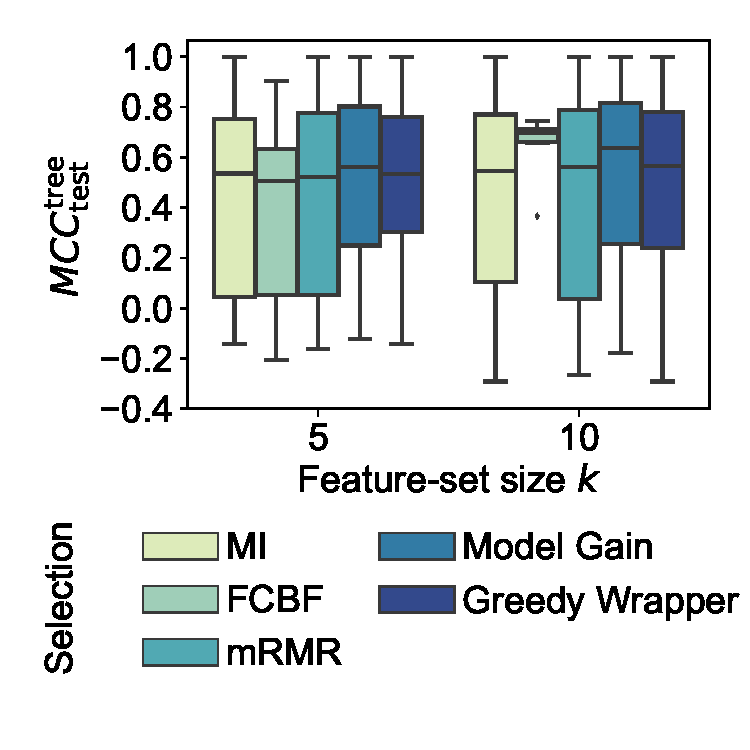
\includegraphics[width=\textwidth, trim=15 35 5 15, clip]{plots/afs-impact-fs-method-k-decision-tree-test-mcc.pdf}
		\caption{Test-set prediction performance by feature-set size~$k$.}
		\label{fig:afs:impact-fs-method-k-decision-tree-test-mcc}
	\end{subfigure}
	\hfill
	\begin{subfigure}[t]{0.48\textwidth}
		\centering
		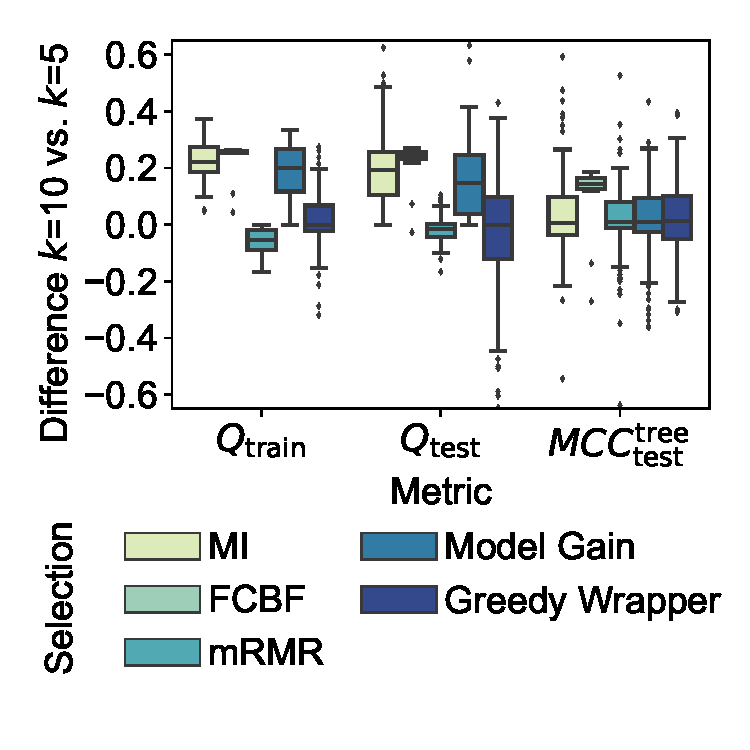
\includegraphics[width=\textwidth, trim=15 35 5 15, clip]{plots/afs-impact-fs-method-k-metric-diff.pdf}
		\caption{
			Difference in feature-set quality between $k=10$ and $k=5$ by evaluation metric.
			Y-axis is truncated to improve readability.
		}
		\label{fig:afs:impact-fs-method-k-metric-diff}
	\end{subfigure}
	\caption{
		Distribution of feature-set quality over datasets and cross-validation folds, by feature-selection method.
		Results from the original feature sets of solver-based sequential search.
	}
	\label{fig:afs:impact-fs-method-k-quality}
\end{figure}

\paragraph{Prediction performance}

The five feature-selection methods in our experiments employ different objective functions~$Q(s,X,y)$, so comparing objective values between them does not make sense.
However, we can analyze the prediction performance of the obtained feature sets.
Figure~\ref{fig:afs:impact-fs-method-k-decision-tree-test-mcc} displays the distribution of a decision tree's test-set MCC on the original feature sets, i.e., without constraints, for the feature-selection methods.
The mean test-set MCC is 0.53 for \emph{Model Gain} and \emph{Greedy Wrapper}, 0.47 for \emph{MI}, 0.46 for \emph{mRMR}, and 0.43 for \emph{FCBF}.
Thus, the analyses of alternative feature sets in Sections~\ref{sec:afs:evaluation:search-methods} and~\ref{sec:afs:evaluation:parameters} focus on \emph{Model Gain} while still discussing the remaining feature-selection methods.

The univariate, model-free method \emph{MI} keeps up surprisingly well with more sophisticated methods.
It uses the same objective function as \emph{Model Gain} but obtains its feature qualities from a bivariate dependency measure rather than a prediction model.

\emph{Greedy Wrapper} uses prediction performance to assess feature-set quality but employs a search heuristic instead of optimizing globally.
In particular, it performed 661 iterations on average to determine the original feature sets.
However, the number of possible feature sets is higher, e.g., already $\binom{15}{5} = 3003$ for the lowest-dimensional dataset in our evaluation (cf.~Table~\ref{tab:afs:datasets}) and $k=5$.
The still high prediction performance comes at the expense of high runtime (cf.~Table~\ref{tab:afs:impact-search-fs-method-optimization-time}), so we prefer \emph{Model Gain} for later evaluations.

\emph{FCBF}'s results may be taken with a grain of salt:
The original feature set in solver-based sequential search is already infeasible, i.e., no solution satisfied the constraints, in 71\% of the cases for \emph{FCBF} but never for the other feature-selection methods.
Over all solver-based search runs, even 89\% of the feature sets were infeasible for \emph{FCBF} but only 18\% for \emph{Model Gain}.
In particular, the combination of feature-correlation constraints in our formulation of \emph{FCBF} (cf.~Equation~\ref{eq:afs:fcbf}) with a cardinality constraint (cf.~Equation~\ref{eq:syn:cardinality}), i.e., enforcing a feature-set size~$k$, may make the problem infeasible, especially if~$k$ gets larger.

\paragraph{Influence of feature-set size~$k$}

One could expect larger feature sets to exhibit a higher feature-set quality than smaller ones, but the picture in our experiments is more nuanced.
In particular, quality may not increase proportionally with $k$ or may even decrease.
As Figure~\ref{fig:afs:impact-fs-method-k-metric-diff} shows for the original feature sets of solver-based sequential search, \emph{MI} and \emph{Model Gain} exhibit an increase of the training-set objective value~$Q_\text{train}$ from~$k=5$ to~$k=10$, i.e., the difference depicted in Figure~\ref{fig:afs:impact-fs-method-k-metric-diff} is positive.
As these objectives are monotonic and the feature qualities are non-negative, a decrease in the training-set objective value is impossible.
In contrast, \emph{Greedy Wrapper} with its black-box objective does not necessarily benefit from more features.
The latter insight also applies to \emph{mRMR}, which normalizes its objective with the number of selected features and penalizes feature redundancy.
For \emph{FCBF}, the fraction of feasible feature sets changes considerably from $k=5$ to $k=10$, so the overall quality between these two settings should not be compared.
As Figure~\ref{fig:afs:impact-fs-method-k-metric-diff} also displays, the benefit of larger feature sets is even less clear for prediction performance.
In particular, all feature-selection methods except \emph{FCBF} show a median difference in test-set MCC close to zero when comparing $k=5$ to $k=10$.

\subsection{Search Methods for Alternatives}
\label{sec:afs:evaluation:search-methods}

\begin{figure}[t]
	\centering
	\begin{subfigure}[t]{\textwidth}
		\centering
		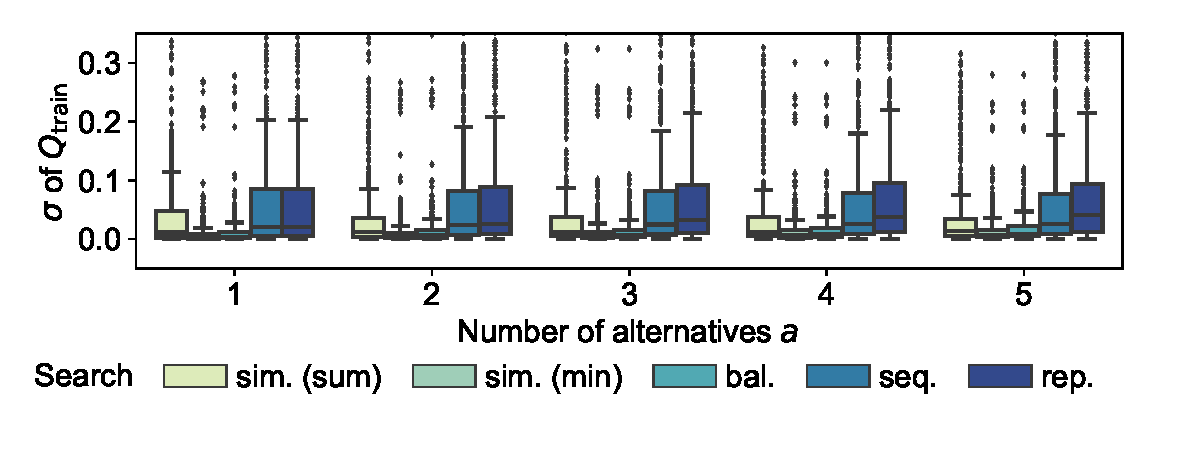
\includegraphics[width=\textwidth, trim=15 25 35 15, clip]{plots/afs-impact-search-stddev-train-objective.pdf}
		\caption{Training-set objective value.}
		\label{fig:afs:impact-search-stddev-train-objective}
	\end{subfigure}
	\\ \vspace{\baselineskip}
	\begin{subfigure}[t]{\textwidth}
		\centering
		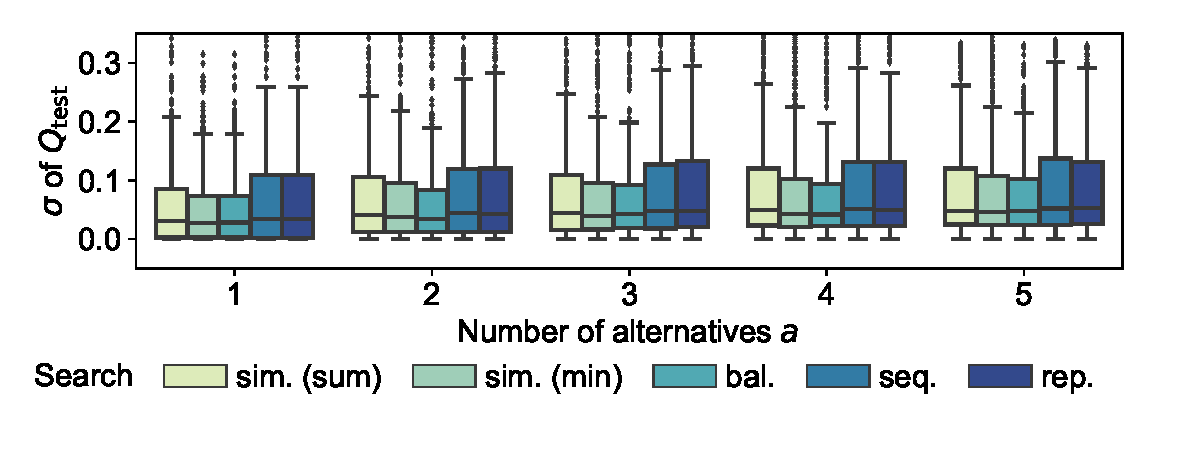
\includegraphics[width=\textwidth, trim=15 25 35 15, clip]{plots/afs-impact-search-stddev-test-objective.pdf}
		\caption{Test-set objective value.}
		\label{fig:afs:impact-search-stddev-test-objective}
	\end{subfigure}
	\\ \vspace{\baselineskip}
	\begin{subfigure}[t]{\textwidth}
		\centering
		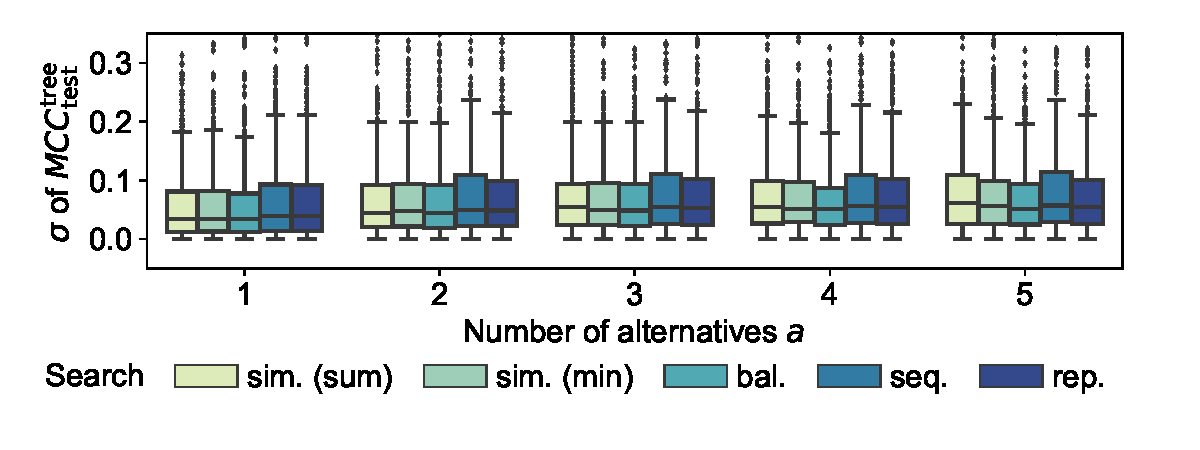
\includegraphics[width=\textwidth, trim=15 25 35 15, clip]{plots/afs-impact-search-stddev-decision-tree-test-mcc.pdf}
		\caption{Test-set prediction performance.}
		\label{fig:afs:impact-search-stddev-decision-tree-test-mcc}
	\end{subfigure}
	\caption{
		Distribution of standard deviation of feature-set quality within search runs over datasets, cross-validation-folds, and~$\tau$, by search method for alternatives and number of alternatives~$a$.
		Results with \emph{Model Gain} as the feature-selection method and $k=5$.
		Excludes search settings where at least one combination of search method and~$a$ yielded no valid solution.
		Y-axes are truncated to improve readability.
	}
	\label{fig:afs:impact-search-stddev-quality}
\end{figure}

\paragraph{Variance in feature-set quality}

As expected, the search method influences how much the training-set objective value~$Q$ varies between multiple alternatives obtained for the same experimental settings, i.e., within one search run for alternatives.
Figure~\ref{fig:afs:impact-search-stddev-train-objective} visualizes this result for \emph{Model Gain} as the feature-selection method and $k=5$.
The figure shows how the standard deviation of the training-set objective value within individual search runs for alternatives is distributed over other experimental settings, e.g., datasets and cross-validation folds.
In particular, the quality of multiple alternatives varies more if they are found by solver-based sequential search rather than solver-based simultaneous search.
For solver-based simultaneous search, min-aggregation yields considerably more homogeneous feature-set quality than sum-aggregation.
These findings apply to all white-box feature-selection methods but not \emph{Greedy Wrapper}.

The heuristic search method \emph{Greedy Balancing} yields a small variance of training-set objective value within search runs, only slightly higher than for solver-based simultaneous search with min-aggregation.
In contrast, \emph{Greedy Replacement} rather mimics solver-based sequential search, having a substantial variance of quality.
Additionally, the variance of \emph{Greedy Replacement} noticeably grows with the number of alternatives~$a$.

As Figures~\ref{fig:afs:impact-search-stddev-test-objective} and~\ref{fig:afs:impact-search-stddev-decision-tree-test-mcc} show, the variance of feature-set quality differs considerably less between the search methods on the test set, for the objective value as well as prediction performance.
This effect might result from overfitting:
Even if the training-set quality is similar, some alternatives might generalize better than others.
Thus, this variance caused by overfitting could alleviate the effect caused by the choice of search method.

\begin{figure}[t]
	\centering
	\begin{subfigure}[t]{\textwidth}
		\centering
		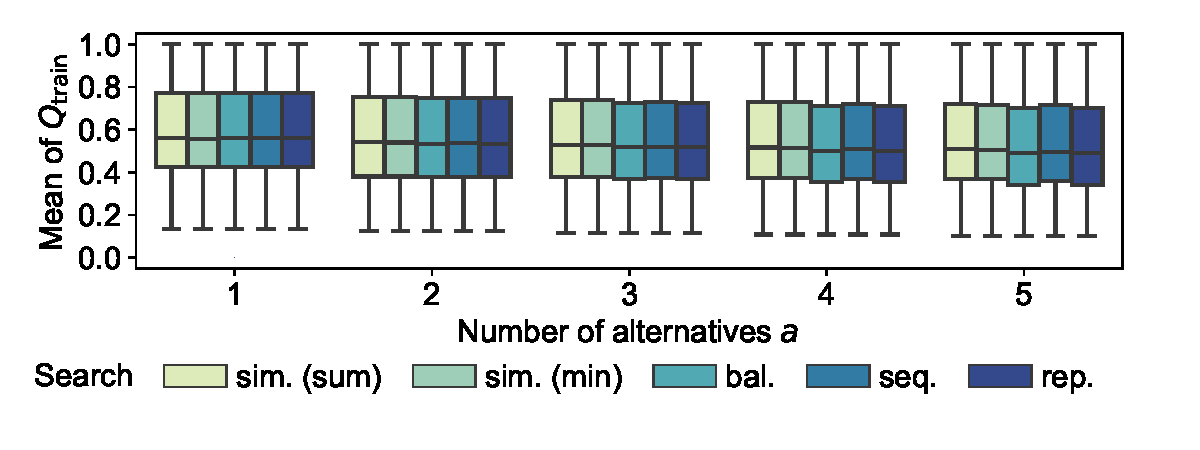
\includegraphics[width=\textwidth, trim=15 25 35 15, clip]{plots/afs-impact-search-mean-train-objective.pdf}
		\caption{Training-set objective value.}
		\label{fig:afs:impact-search-mean-train-objective}
	\end{subfigure}
	\\ \vspace{\baselineskip}
	\begin{subfigure}[t]{\textwidth}
		\centering
		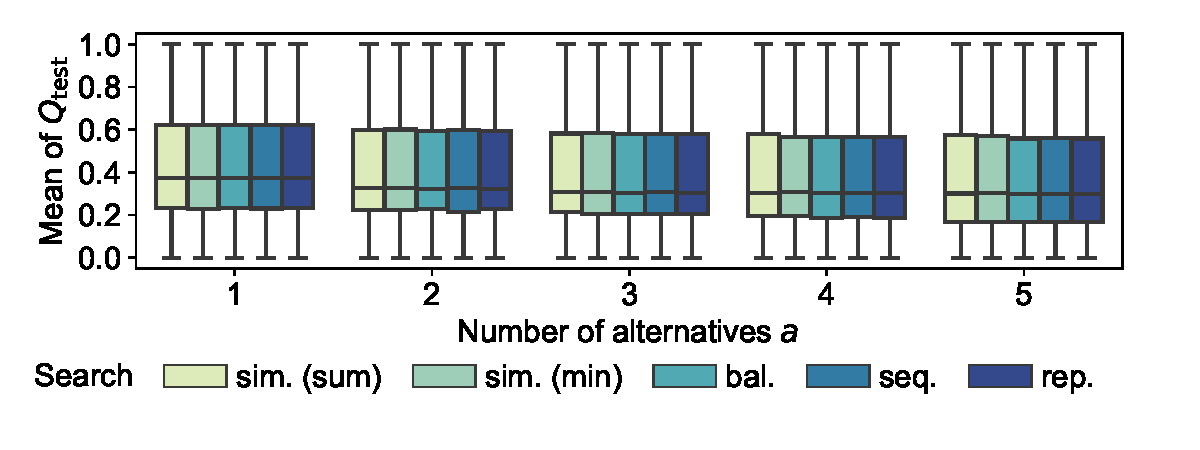
\includegraphics[width=\textwidth, trim=15 25 35 15, clip]{plots/afs-impact-search-mean-test-objective.pdf}
		\caption{Test-set objective value.}
		\label{fig:afs:impact-search-mean-test-objective}
	\end{subfigure}
	\\ \vspace{\baselineskip}
	\begin{subfigure}[t]{\textwidth}
		\centering
		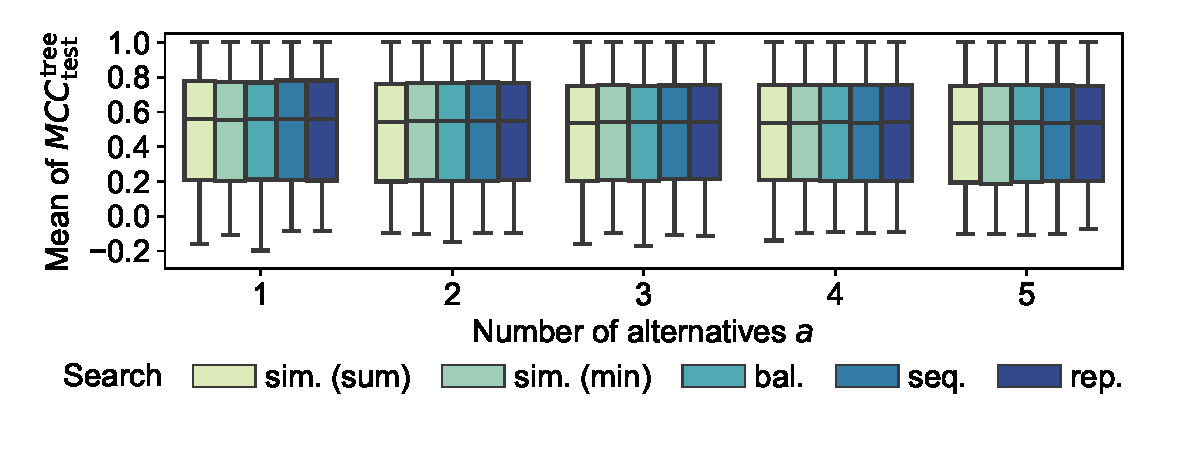
\includegraphics[width=\textwidth, trim=15 25 35 14, clip]{plots/afs-impact-search-mean-decision-tree-test-mcc.pdf}
		\caption{Test-set prediction performance.}
		\label{fig:afs:impact-search-mean-decision-tree-test-mcc}
	\end{subfigure}
	\caption{
		Distribution of mean feature-set quality within search runs over datasets, cross-validation-folds, and~$\tau$, by search method for alternatives and number of alternatives~$a$.
		Results with \emph{Model Gain} as the feature-selection method and $k=5$.
		Excludes search settings where at least one combination of search method and~$a$ yielded no valid solution.
		Y-axes are truncated to improve readability.
	}
	\label{fig:afs:impact-search-mean-quality}
\end{figure}

\paragraph{Average value of feature-set quality}

While obtaining alternatives of homogeneous quality can be one goal of simultaneous search, another selling point would be obtaining alternatives of higher average quality than sequential search.
However, this potential advantage rarely materialized in our experiments.
In particular, Figure~\ref{fig:afs:impact-search-mean-train-objective} compares the distribution of the mean training-set objective value in search runs with \emph{Model Gain} as the feature-selection method and $k=5$.
We observe that all search methods yield very similar overall distributions of average feature-set quality.
Comparing solver-based sequential and simultaneous search on each experimental setting separately and then aggregating also shows a mean quality difference close to zero.
Further, outliers can occur in both directions, i.e., either solver-based search method may yield higher quality.

The mean test-set objective value in Figure~\ref{fig:afs:impact-search-mean-test-objective} and the mean test-set prediction performance in Figure~\ref{fig:afs:impact-search-mean-decision-tree-test-mcc} also exhibit a negligible quality difference between the search methods.
Finally, the other four feature-selection methods besides \emph{Model Gain} do not show a general quality advantage of solver-based simultaneous search either.

\begin{figure}[t]
	\centering
	\begin{subfigure}[t]{0.48\textwidth}
		\centering
		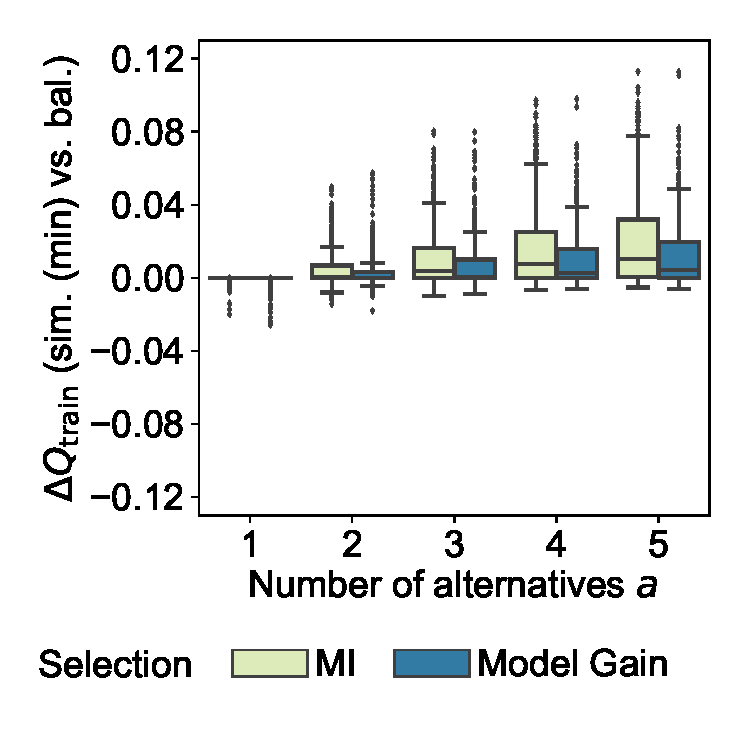
\includegraphics[width=\textwidth, trim=15 30 15 15, clip]{plots/afs-impact-search-heuristics-metric-diff-sim-num-alternatives.pdf}
		\caption{
			Difference between solver-based simultaneous (min-aggregation) search and \emph{Greedy Balancing}, by the number of alternatives~$a$.
		}
		\label{fig:afs:impact-search-heuristics-metric-diff-sim-num-alternatives}
	\end{subfigure}
	\hfill
	\begin{subfigure}[t]{0.48\textwidth}
		\centering
		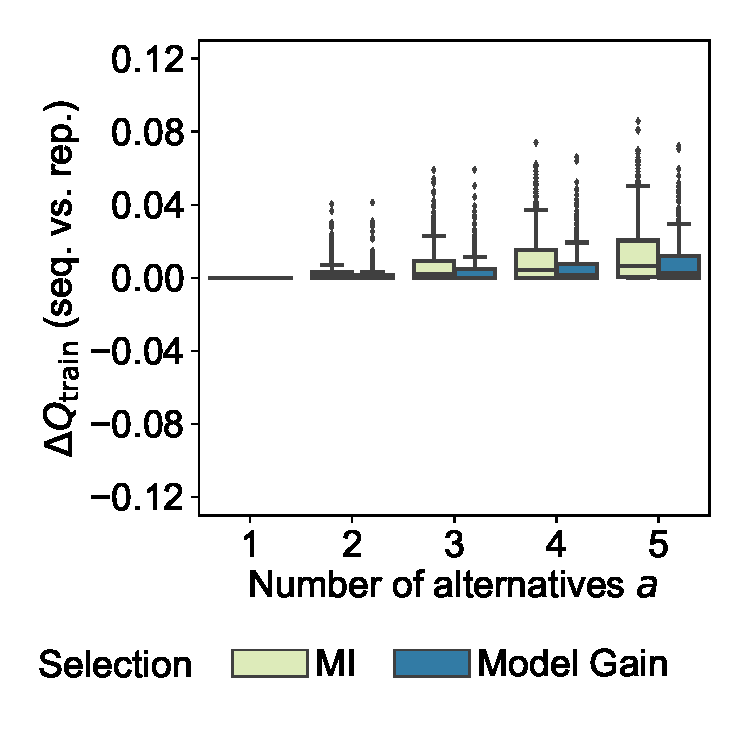
\includegraphics[width=\textwidth, trim=15 30 15 15, clip]{plots/afs-impact-search-heuristics-metric-diff-seq-num-alternatives.pdf}
		\caption{
			Difference between solver-based sequential search and \emph{Greedy Replacement}, by the number of alternatives~$a$.
		}
		\label{fig:afs:impact-search-heuristics-metric-diff-seq-num-alternatives}
	\end{subfigure}
	\\ \vspace{\baselineskip}
	\begin{subfigure}[t]{0.48\textwidth}
		\centering
		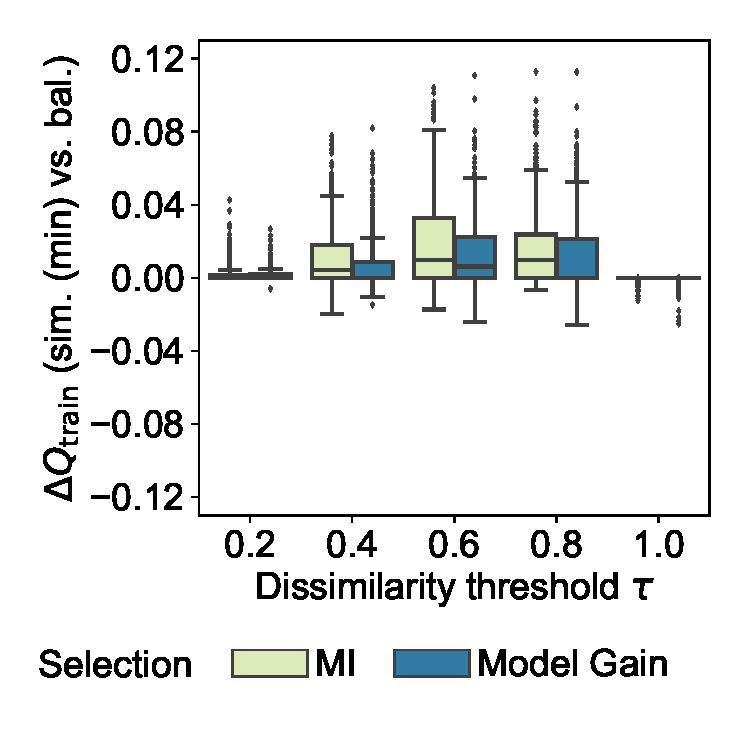
\includegraphics[width=\textwidth, trim=15 30 15 15, clip]{plots/afs-impact-search-heuristics-metric-diff-sim-tau.pdf}
		\caption{
			Difference between solver-based simultaneous (min-aggregation) search and \emph{Greedy Balancing}, by the dissimilarity threshold~$\tau$.
		}
		\label{fig:afs:impact-search-heuristics-metric-diff-sim-tau}
	\end{subfigure}
	\hfill
	\begin{subfigure}[t]{0.48\textwidth}
		\centering
		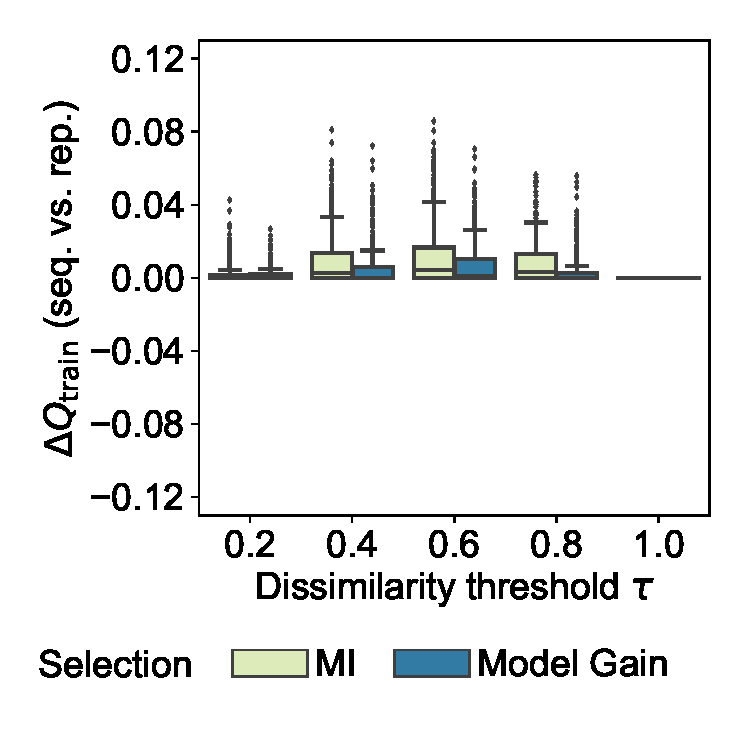
\includegraphics[width=\textwidth, trim=15 30 15 15, clip]{plots/afs-impact-search-heuristics-metric-diff-seq-tau.pdf}
		\caption{
			Difference between solver-based sequential search and \emph{Greedy Replacement}, by the dissimilarity threshold~$\tau$.
		}
		\label{fig:afs:impact-search-heuristics-metric-diff-seq-tau}
	\end{subfigure}
	\caption{
		Distribution of difference in mean training feature-set quality within a search run between solver-based and heuristic search methods over remaining experimental settings, by feature-selection method.
		Results with $k=5$.
		Excludes search settings where at least one combination of search method and~$a$ yielded no valid solution.
	}
	\label{fig:afs:impact-search-heuristics-metric-diff}
\end{figure}

\paragraph{Quality difference of heuristics}

We now look closer at the quality difference between solver-based and heuristic search.
Figure~\ref{fig:afs:impact-search-heuristics-metric-diff} compares the mean training feature-set quality within search runs for each experimental setting separately.
In particular, we compare solver-based simultaneous search with min-aggregation to \emph{Greedy Balancing} (cf.~Figures~\ref{fig:afs:impact-search-heuristics-metric-diff-sim-num-alternatives} and~\ref{fig:afs:impact-search-heuristics-metric-diff-sim-tau}) and solver-based sequential search to \emph{Greedy Replacement} (cf.~Figures~\ref{fig:afs:impact-search-heuristics-metric-diff-seq-num-alternatives} and~\ref{fig:afs:impact-search-heuristics-metric-diff-seq-tau}).
Positive values in Figure~\ref{fig:afs:impact-search-heuristics-metric-diff} express that solver-based search yields higher quality; negative values favor heuristic search.
The latter can occur if solver-based search yields suboptimal solutions due to timeouts, as we analyze later (cf.~Table~\ref{tab:afs:impact-search-fs-method-optimization-status}).

Figures~\ref{fig:afs:impact-search-heuristics-metric-diff-sim-num-alternatives} and~\ref{fig:afs:impact-search-heuristics-metric-diff-seq-num-alternatives} compare solver-based and heuristic search over the number of alternatives~$a$.
For $a=1$, solver-based and heuristic search yield the same mean training feature-set quality except when timeouts occur.
The more alternatives are desired, the more advantageous a solver-based search is quality-wise.
As in prior analyses, the picture is less clear on the test set, which shows a smaller quality difference here.
Further, the difference in mean training feature-set quality between \emph{Greedy Balancing} and solver-based simultaneous search (cf.~Figure~\ref{fig:afs:impact-search-heuristics-metric-diff-sim-num-alternatives}) grows faster with~$a$ than between \emph{Greedy Replacement} and solver-based sequential search (cf.~Figure~\ref{fig:afs:impact-search-heuristics-metric-diff-seq-num-alternatives}).
As an explanation, consider that optimal simultaneous search may generally develop a quality advantage over optimal sequential search for more alternatives.
\emph{Greedy Balancing} selects the same features as \emph{Greedy Replacement}, i.e., a sequential search heuristic, and only distributes them differently into feature sets, yielding the same mean feature-set quality.

Figures~\ref{fig:afs:impact-search-heuristics-metric-diff-sim-tau} and~\ref{fig:afs:impact-search-heuristics-metric-diff-seq-tau} compare solver-based and heuristic search over the dissimilarity threshold~$\tau$.
Unlike for~$a$, the difference in mean training feature-set quality between solver-based and heuristic search does not increase over the whole range of~$\tau$ but shows an increase followed by a decrease.
In particular, $\tau=1$ allows the two heuristic search methods to reach the same mean training feature-set quality as the solver-based methods.
This observation corresponds to our theoretical result that optimizing the summed quality of alternatives with~$\tau=1$ admits polynomial-time algorithms (cf.~Proposition~\ref{prop:afs:complexity-partitioning-sum}).

\begin{table}[t]
	\centering
	\caption{
		Frequency of optimization statuses (cf.~Section~\ref{sec:afs:experimental-design:evaluation}) over datasets, cross-validation folds, $a$, and $\tau$, by feature-selection method and search method for alternatives.
		Results with $k=5$, $a \in \{1,2,3,4,5\}$, and excluding \emph{Greedy Wrapper}, which does not use the solver for optimizing.
		Each row adds up to 100\%.
	}
	\begin{tabular}{llrrrr}
		\toprule
		\multirow{2}{*}{Feature selection} & \multirow{2}{*}{Search} & \multicolumn{4}{c}{Optimization status} \\
		\cmidrule(lr){3-6}
		& & Infeasible & Not solved & Feasible & Optimal \\
		\midrule
		FCBF & seq. & 74.51\% & 0.00\% & 0.00\% & 25.49\% \\
		FCBF & sim. (min) & 73.07\% & 0.00\% & 1.60\% & 25.33\% \\
		FCBF & sim. (sum) & 73.07\% & 0.00\% & 2.19\% & 24.75\% \\
		MI & bal. & 0.00\% & 9.20\% & 90.80\% & 0.00\% \\
		MI & rep. & 0.00\% & 9.20\% & 90.80\% & 0.00\% \\
		MI & seq. & 4.93\% & 0.00\% & 0.00\% & 95.07\% \\
		MI & sim. (min) & 4.67\% & 0.00\% & 9.33\% & 86.00\% \\
		MI & sim. (sum) & 4.67\% & 0.00\% & 3.04\% & 92.29\% \\
		Model Gain & bal. & 0.00\% & 9.20\% & 90.80\% & 0.00\% \\
		Model Gain & rep. & 0.00\% & 9.20\% & 90.80\% & 0.00\% \\
		Model Gain & seq. & 4.93\% & 0.00\% & 0.00\% & 95.07\% \\
		Model Gain & sim. (min) & 4.67\% & 0.00\% & 5.28\% & 90.05\% \\
		Model Gain & sim. (sum) & 4.67\% & 0.00\% & 1.87\% & 93.47\% \\
		mRMR & seq. & 4.88\% & 0.00\% & 9.55\% & 85.57\% \\
		mRMR & sim. (min) & 4.67\% & 0.00\% & 48.64\% & 46.69\% \\
		mRMR & sim. (sum) & 4.67\% & 0.00\% & 67.04\% & 28.29\% \\
		\bottomrule
	\end{tabular}
	\label{tab:afs:impact-search-fs-method-optimization-status}
\end{table}

\begin{table}[t]
	\centering
	\caption{
		Frequency of optimization statuses (cf.~Section~\ref{sec:afs:experimental-design:evaluation}) over datasets, cross-validation folds, feature-selection methods, and~$\tau$, by number of alternatives~$a$.
		Results from solver-based simultaneous search with sum-aggregation, $k=5$, and excluding \emph{Greedy Wrapper}.
		Each row adds up to 100\%.
	}
	\begin{tabular}{rrrr}
		\toprule
		\multirow{2}{*}{$a$} & \multicolumn{3}{c}{Optimization status} \\
		\cmidrule(lr){2-4}
		& Infeasible & Feasible & Optimal \\
		\midrule
		1 & 16.10\% & 7.60\% & 76.30\% \\
		2 & 17.50\% & 13.27\% & 69.23\% \\
		3 & 20.00\% & 20.20\% & 59.80\% \\
		4 & 27.00\% & 21.43\% & 51.57\% \\
		5 & 28.23\% & 30.17\% & 41.60\% \\
		\bottomrule
	\end{tabular}
	\label{tab:afs:impact-num-alternatives-optimization-status}
\end{table}

\paragraph{Optimization status}

Suboptimal search results are one reason why solver-based simultaneous search fails to consistently beat solver-based sequential search quality-wise.
For \emph{Greedy Wrapper}, the search is heuristic per se and does not cover the entire search space.
For all feature-selection methods, the solver can time out.
Table~\ref{tab:afs:impact-search-fs-method-optimization-status} shows that solver-based simultaneous search has a higher likelihood of timeouts than solver-based sequential search, likely due to the larger size of the optimization problem (cf.~Table~\ref{tab:afs:seq-sim-comparison}).
In particular, for up to five alternatives and $k=5$, all solver-based sequential searches for \emph{FCBF}, \emph{MI}, and \emph{Model Gain} finished within the timeout, i.e., yielded the optimal feature set or ascertained infeasibility, while \emph{mRMR} had about 10\% timeouts.
In contrast, for solver-based simultaneous search with sum-aggregation, all feature-selection methods experience timeouts:
1--3\% of the searches for \emph{FCBF}, \emph{MI}, and \emph{Model Gain}, and 67\% of the searches for \emph{mRMR} found a feasible solution but could not prove optimality.
Such timeout-affected simultaneous solutions can be worse than optimal sequential solutions.

\emph{mRMR} is especially prone to suboptimal solutions, likely because it has a more complex objective (cf.~Equation~\ref{eq:afs:mrmr-linear}) than~\emph{MI} and \emph{Model Gain}.
\emph{FCBF} often results in infeasible optimization problems since its constraints, which prevent the selection of redundant features (cf.~Equation~\ref{eq:afs:fcbf}), might prevent finding any valid feature set of size~$k$.
Min-aggregation instead of sum-aggregation in solver-based simultaneous search exhibits more timeouts for \emph{MI} and \emph{Model Gain} but less for \emph{FCBF} and \emph{mRMR}.
Still, solver-based sequential search incurs fewer timeouts for all of these four feature-selection methods.

Also, note that the fraction of timeouts in solver-based simultaneous search strongly depends on the number of alternatives~$a$, as Table~\ref{tab:afs:impact-num-alternatives-optimization-status} displays:
For $k=5$ and sum-aggregation, roughly 8\% of the white-box searches timed out for~$a=1$, but 20\% for~$a=3$ and 30\% for~$a=5$.
While we grant solver-based simultaneous searches proportionally more time for multiple alternatives (cf.~Section~\ref{sec:afs:experimental-design:approaches:alternatives}), the observed increase in timeouts suggests that runtime increases super-proportionally with~$a$, as we analyze later.

For the heuristic search methods, Table~\ref{tab:afs:impact-search-fs-method-optimization-status} shows that \emph{Greedy Replacement} more often did not find a valid alternative (9.20\%) than solver-based sequential search (4.93\%).
A similar phenomenon occurred for \emph{Greedy Balancing} (9.20\%) compared to solver-based simultaneous search (4.67\%).
Such a result can be expected since both heuristic search methods stop early as soon as each feature is part of at least one alternative.

\begin{table}[t]
	\centering
	\caption{
		Mean optimization time over datasets, cross-validation folds, $a$, and $\tau$, by feature-selection method and search method for alternatives.
		Results with $k=5$ and $a \in \{1,2,3,4,5\}$.
	}
	\begin{tabular}{lrrrrr}
		\toprule
		\multirow{2}{*}{Feature selection} & \multicolumn{5}{c}{Optimization time} \\
		\cmidrule(lr){2-6}
		& Bal. & Rep. & Seq. & Sim. (min) & Sim. (sum) \\
		\midrule
		FCBF & --- & --- & 0.22~s & 11.41~s & 12.62~s \\
		Greedy Wrapper & --- & --- & 52.62~s & 68.39~s & 70.36~s \\
		MI & 0.00~s & 0.00~s & 0.03~s & 47.39~s & 24.56~s \\
		Model Gain & 0.00~s & 0.00~s & 0.03~s & 30.38~s & 19.08~s \\
		mRMR & --- & --- & 33.59~s & 156.00~s & 189.25~s \\
		\bottomrule
	\end{tabular}
	\label{tab:afs:impact-search-fs-method-optimization-time}
\end{table}

\begin{table}[t]
	\centering
	\caption{
		Mean optimization time over datasets, cross-validation folds, and $\tau$, by number of alternatives and feature-selection method.
		Results from solver-based simultaneous search with sum-aggregation and $k=5$.
	}
	\begin{tabular}{lrrrrr}
		\toprule
		\multirow{2}{*}{$a$} & \multicolumn{5}{c}{Optimization time} \\
		\cmidrule(lr){2-6}
		& FCBF & Greedy Wrapper & MI & Model Gain & mRMR \\
		\midrule
		1 & 0.45~s & 28.44~s & 0.03~s & 0.02~s & 44.68~s \\
		2 & 0.86~s & 41.76~s & 0.09~s & 0.08~s & 117.62~s \\
		3 & 2.97~s & 62.70~s & 0.30~s & 0.27~s & 208.14~s \\
		4 & 13.32~s & 96.65~s & 3.68~s & 3.47~s & 258.19~s \\
		5 & 45.52~s & 122.26~s & 118.72~s & 91.58~s & 317.63~s \\
		\bottomrule
	\end{tabular}
	\label{tab:afs:impact-num-alternatives-fs-method-optimization-time}
\end{table}

\paragraph{Optimization time}

As Table~\ref{tab:afs:impact-search-fs-method-optimization-time} shows, solver-based sequential search is faster on average than solver-based simultaneous search for all five feature-selection methods.
In particular, the difference is up to three orders of magnitude for the four white-box feature-selection methods.
Further, \emph{FCBF}, \emph{MI}, and \emph{Model Gain} experience a dramatic increase in optimization time with the number of alternatives~$a$ in solver-based simultaneous search, as Table~\ref{tab:afs:impact-num-alternatives-fs-method-optimization-time} displays.
In contrast, the runtime increase is considerably less for solver-based sequential search, which shows an approximately linear trend with the number of alternatives.

Table~\ref{tab:afs:impact-search-fs-method-optimization-time} also shows that the optimization time of the heuristic search methods for \emph{MI} and \emph{Model Gain} is negligible.
In particular, \emph{Greedy Replacement} and \emph{Greedy Balancing} never took longer than 1~ms per search run for alternatives.
These results highlight the runtime advantage of the heuristics, particularly of \emph{Greedy Balancing} for simultaneous search.

An interesting question for practitioners is how the runtime relates to~$n$, the number of features in the dataset.
One could expect a positive correlation since the problem instance increases with~$n$.
Roughly speaking, this trend appears in our experimental data indeed.
However, the observed trend is rather noisy, particularly for solver-based simultaneous search, and some higher-dimensional datasets even show lower average runtimes than lower-dimensional ones.
This result indicates that other factors than~$n$ influence runtime as well, e.g., other experimental settings or the solver's internal search heuristics.

Based on all results described in this section, we focus on solver-based sequential search in the next section.
In particular, it was significantly faster than solver-based simultaneous search while yielding similar feature-set quality.

\subsection{User Parameters \texorpdfstring{$a$ And $\tau$}{}}
\label{sec:afs:evaluation:parameters}

\begin{figure}[p]
	\centering
	\begin{subfigure}[t]{0.48\textwidth}
		\centering
		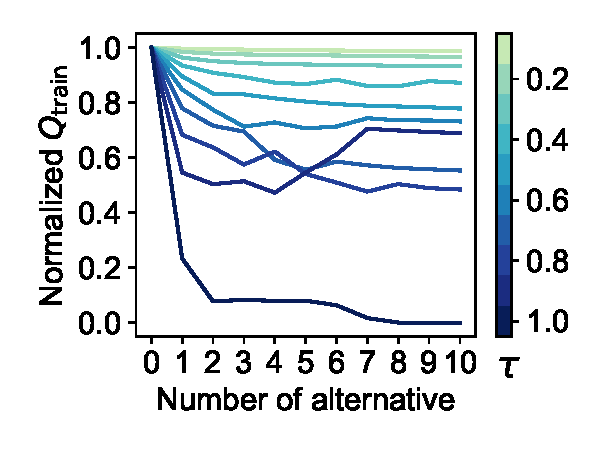
\includegraphics[width=\textwidth, trim=15 17 10 15, clip]{plots/afs-impact-num-alternatives-tau-train-objective-max.pdf}
		\caption{
			Training-set objective value.
			Infeasible feature sets excluded.
		}
		\label{fig:afs:impact-num-alternatives-tau-train-objective-max}
	\end{subfigure}
	\hfill
	\begin{subfigure}[t]{0.48\textwidth}
		\centering
		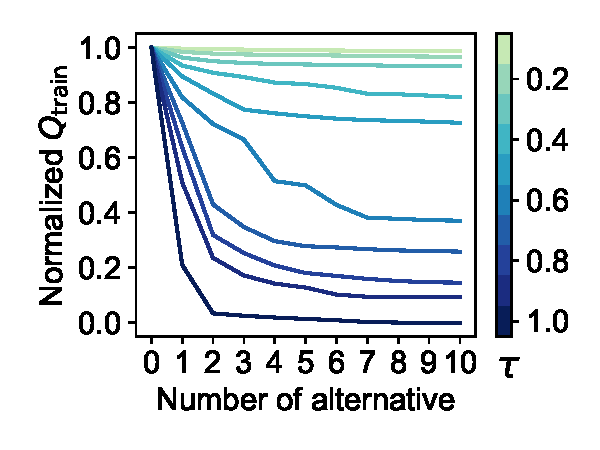
\includegraphics[width=\textwidth, trim=15 17 10 15, clip]{plots/afs-impact-num-alternatives-tau-train-objective-max-fillna.pdf}
		\caption{
			Training-set objective value.
			Infeasible feature sets assigned a quality of~0.
		}
		\label{fig:afs:impact-num-alternatives-tau-train-objective-max-fillna}
	\end{subfigure}
	\\ \vspace{\baselineskip}
	\begin{subfigure}[t]{0.48\textwidth}
		\centering
		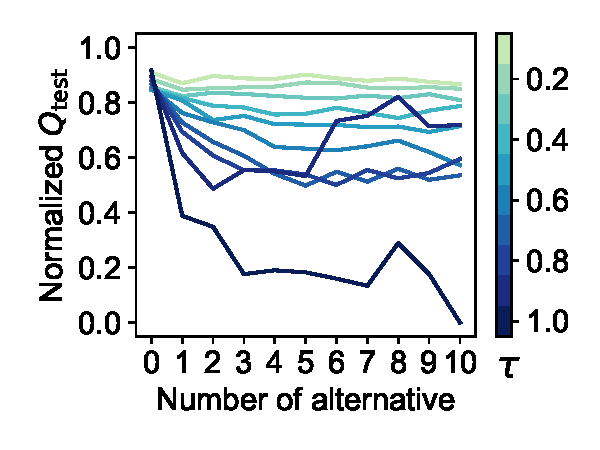
\includegraphics[width=\textwidth, trim=15 17 10 15, clip]{plots/afs-impact-num-alternatives-tau-test-objective-max.pdf}
		\caption{
			Test-set objective value.
			Infeasible feature sets excluded.
		}
		\label{fig:afs:impact-num-alternatives-tau-test-objective-max}
	\end{subfigure}
	\hfill
	\begin{subfigure}[t]{0.48\textwidth}
		\centering
		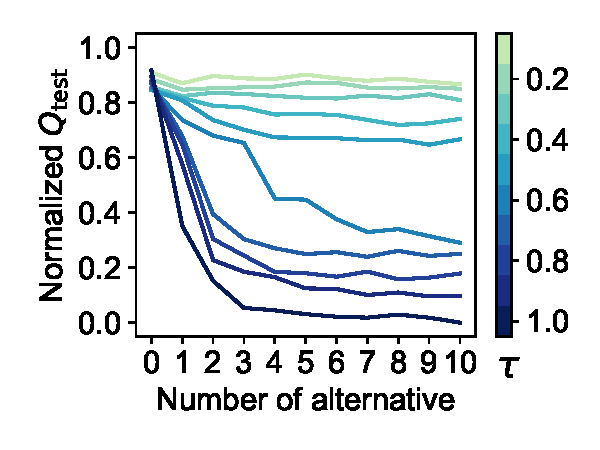
\includegraphics[width=\textwidth, trim=15 17 10 15, clip]{plots/afs-impact-num-alternatives-tau-test-objective-max-fillna.pdf}
		\caption{
			Test-set objective value.
			Infeasible feature sets assigned a quality of~0.
		}
		\label{fig:afs:impact-num-alternatives-tau-test-objective-max-fillna}
	\end{subfigure}
	\\ \vspace{\baselineskip}
	\begin{subfigure}[t]{0.48\textwidth}
		\centering
		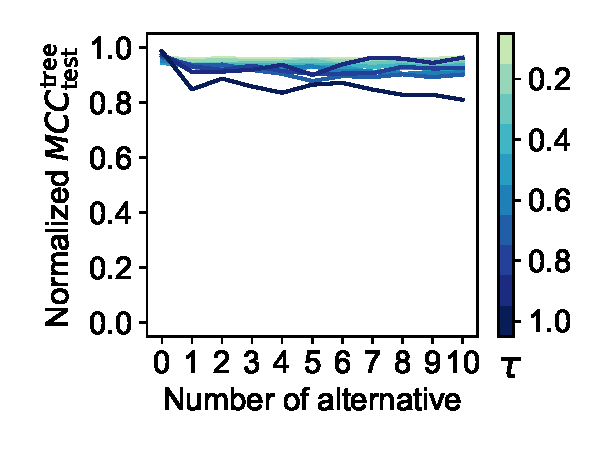
\includegraphics[width=\textwidth, trim=15 17 10 15, clip]{plots/afs-impact-num-alternatives-tau-decision-tree-test-mcc-max.pdf}
		\caption{
			Test-set prediction performance.
			Infeasible feature sets excluded.
		}
		\label{fig:afs:impact-num-alternatives-tau-decision-tree-test-mcc-max}
	\end{subfigure}
	\hfill
	\begin{subfigure}[t]{0.48\textwidth}
		\centering
		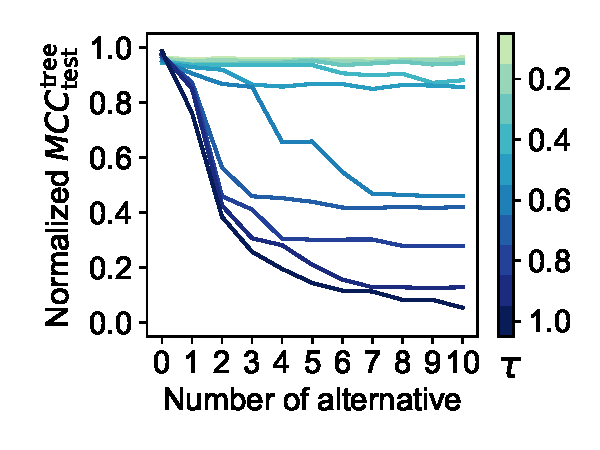
\includegraphics[width=\textwidth, trim=15 17 10 15, clip]{plots/afs-impact-num-alternatives-tau-decision-tree-test-mcc-max-fillna.pdf}
		\caption{
			Test-set prediction performance.
			Infeasible feature sets assigned a quality of~0.
		}
		\label{fig:afs:impact-num-alternatives-tau-decision-tree-test-mcc-max-fillna}
	\end{subfigure}
	\caption{
		Mean feature-set quality over datasets and cross-validation folds, max-normalized per search run for alternatives, by the number of alternative and dissimilarity threshold~$\tau$.
		Results from solver-based sequential search with \emph{Model Gain} as the feature-selection method and $k=10$.
	}
	\label{fig:afs:impact-num-alternatives-tau-quality}
\end{figure}

\paragraph{Feature-set quality}

Higher values of the two user parameters introduce more (for~$a$) or stronger (for~$\tau$) constraints into the optimization problem of alternative feature selection.
Thus, one would expect a corresponding decrease in feature-set quality.
Figure~\ref{fig:afs:impact-num-alternatives-tau-quality} illustrates this trend for \emph{Model Gain} as the feature-selection method and $k=10$.
Since the maximum feature-set quality varies among datasets, we max-normalize quality in this figure.
In particular, we set the highest feature-set quality in each search run for alternatives to~1 and scale the other feature-set qualities accordingly.
For prediction performance in terms of MCC, we shift its range from~$[-1,1]$ to~$[0,1]$ before normalization.

Figure~\ref{fig:afs:impact-num-alternatives-tau-quality} shows that multiple alternatives may have a similar quality.
Further, the training-set objective value (cf.~Figure~\ref{fig:afs:impact-num-alternatives-tau-train-objective-max}) decreases most from the original feature set, i.e., the zeroth alternative, to the first alternative, but less beyond.
Also, the decrease strongly depends on the dissimilarity threshold~$\tau$.
For a low dissimilarity threshold like $\tau=0.1$, the training-set objective value barely drops over the number of alternatives.
Additionally, note that Figure~\ref{fig:afs:impact-num-alternatives-tau-quality} averages the normalized feature-set quality over multiple datasets.
In our experiments, datasets with more features tend to experience a smaller decrease in quality over~$a$ and~$\tau$.
As higher-dimensional datasets offer more options for alternatives, this observation makes sense.
However, this effect is not guaranteed since datasets with many features could also contain many useless features instead of interesting alternatives.

The overall decrease in quality is slightly less pronounced for the test-set objective value (Figure~\ref{fig:afs:impact-num-alternatives-tau-test-objective-max}) than on the training set (Figure~\ref{fig:afs:impact-num-alternatives-tau-train-objective-max}) since overfitting might occur.
In particular, the original feature set can even have lower test-set quality than the subsequent alternatives.
The trend becomes even less clear for prediction performance, which varies little over~$a$ and~$\tau$ in our experiments (cf.~Figure~\ref{fig:afs:impact-num-alternatives-tau-decision-tree-test-mcc-max}).
In general, the optimization objective~$Q$ may only partially indicate actual prediction performance since the former may use a simplified feature-set quality criterion.
Indeed, the correlation between optimization objective~$Q$ and prediction MCC is only weak to moderate in our experiments.

\begin{figure}[t]
	\centering
	\begin{subfigure}[t]{0.48\textwidth}
		\centering
		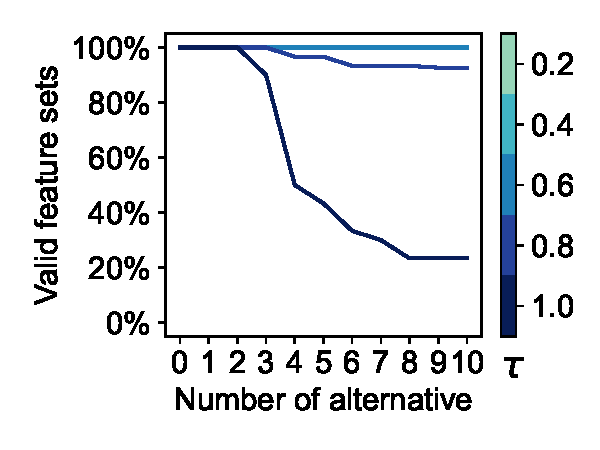
\includegraphics[width=\textwidth, trim=15 15 10 15, clip]{plots/afs-impact-num-alternatives-tau-optimization-status-k-5.pdf}
		\caption{Feature-set size~$k=5$.}
		\label{fig:afs:impact-num-alternatives-tau-optimization-status-k-5}
	\end{subfigure}
	\hfill
	\begin{subfigure}[t]{0.48\textwidth}
		\centering
		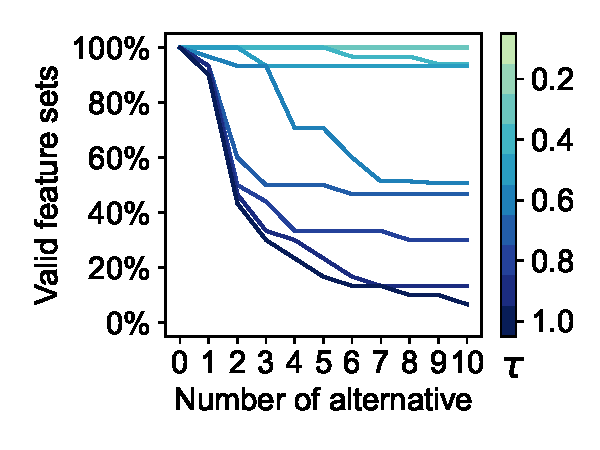
\includegraphics[width=\textwidth, trim=15 15 10 15, clip]{plots/afs-impact-num-alternatives-tau-optimization-status-k-10.pdf}
		\caption{Feature-set size~$k=10$.}
		\label{fig:afs:impact-num-alternatives-tau-optimization-status-k-10}
	\end{subfigure}
	\caption{
		Frequency of optimization runs yielding a valid feature set over datasets and cross-validation folds, by the number of alternative and dissimilarity threshold~$\tau$.
		Results from solver-based sequential search with \emph{Model Gain} as the feature-selection method.
	}
	\label{fig:afs:impact-num-alternatives-tau-optimization-status}
\end{figure}

\paragraph{Optimization status}

The previous observations refer to the quality of the found feature sets.
However, the more alternatives one desires and the more they should differ, the likelier an infeasible optimization problem is.
Figure~\ref{fig:afs:impact-num-alternatives-tau-optimization-status} visualizes the fraction of valid feature sets over the number of alternatives and dissimilarity threshold~$\tau$, showing the expected trend.
Additionally, Figures~\ref{fig:afs:impact-num-alternatives-tau-train-objective-max-fillna},~\ref{fig:afs:impact-num-alternatives-tau-test-objective-max-fillna}, and~\ref{fig:afs:impact-num-alternatives-tau-decision-tree-test-mcc-max-fillna} display the same data as Figures~\ref{fig:afs:impact-num-alternatives-tau-train-objective-max},~\ref{fig:afs:impact-num-alternatives-tau-test-objective-max}, and~\ref{fig:afs:impact-num-alternatives-tau-decision-tree-test-mcc-max} but with the quality of infeasible feature sets set to zero instead of excluding these feature sets from evaluation.
Consequently, the decrease in feature-set quality over~$a$ and~$\tau$ is noticeably stronger.
In contrast, if only considering valid feature sets, the mean quality in our experiments can increase over the number of alternatives, e.g., as visible in Figures~\ref{fig:afs:impact-num-alternatives-tau-train-objective-max} and~\ref{fig:afs:impact-num-alternatives-tau-test-objective-max} for $\tau=0.9$.
This counterintuitive phenomenon can occur because some datasets run out of valid feature sets sooner than others, so the average quality may be determined for different sets of datasets at each number of alternatives.

\begin{figure}[t]
	\centering
	\begin{subfigure}[t]{0.48\textwidth}
		\centering
		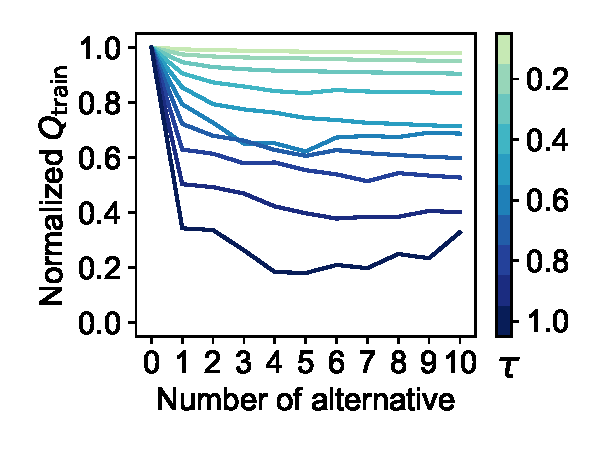
\includegraphics[width=\textwidth, trim=15 17 10 15, clip]{plots/afs-impact-num-alternatives-tau-train-objective-max-mi.pdf}
		\caption{
			\emph{MI} as the feature-selection method.
		}
		\label{fig:afs:impact-num-alternatives-tau-train-objective-max-mi}
	\end{subfigure}
	\hfill
	\begin{subfigure}[t]{0.48\textwidth}
		\centering
		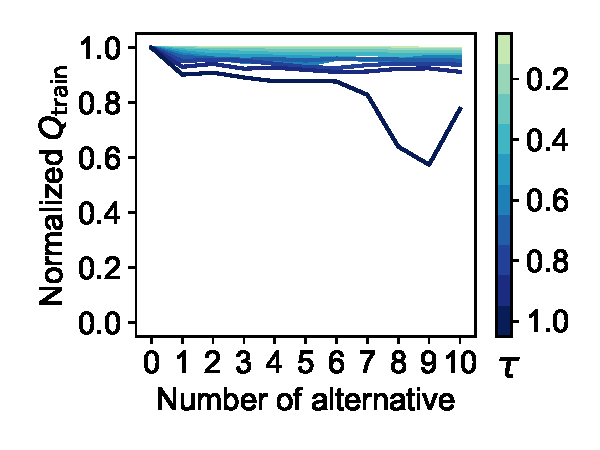
\includegraphics[width=\textwidth, trim=15 17 10 15, clip]{plots/afs-impact-num-alternatives-tau-train-objective-max-mrmr.pdf}
		\caption{
			\emph{mRMR} as the feature-selection method.
		}
		\label{fig:afs:impact-num-alternatives-tau-train-objective-max-mrmr}
	\end{subfigure}
	\\ \vspace{\baselineskip}
	\begin{subfigure}[t]{0.48\textwidth}
		\centering
		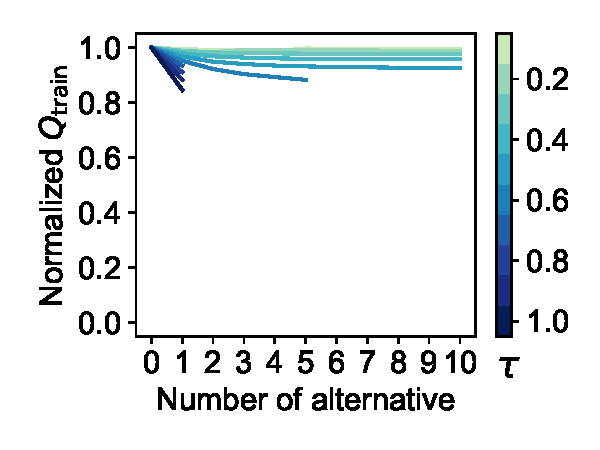
\includegraphics[width=\textwidth, trim=15 17 10 15, clip]{plots/afs-impact-num-alternatives-tau-train-objective-max-fcbf.pdf}
		\caption{
			\emph{FCBF} as the feature-selection method.
		}
		\label{fig:afs:impact-num-alternatives-tau-train-objective-max-fcbf}
	\end{subfigure}
	\hfill
	\begin{subfigure}[t]{0.48\textwidth}
		\centering
		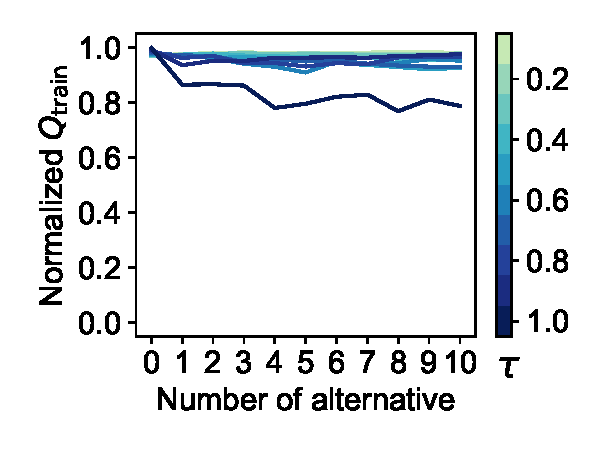
\includegraphics[width=\textwidth, trim=15 17 10 15, clip]{plots/afs-impact-num-alternatives-tau-train-objective-max-greedy-wrapper.pdf}
		\caption{
			\emph{Greedy Wrapper} as the feature-selection method.
		}
		\label{fig:afs:impact-num-alternatives-tau-train-objective-max-greedy-wrapper}
	\end{subfigure}
	\caption{
		Mean training-set objective value over datasets and cross-validation folds, max-normalized per search run for alternatives, by the number of alternative and dissimilarity threshold~$\tau$.
		Results from solver-based sequential search with $k=10$.
		Infeasible feature sets excluded.
	}
	\label{fig:afs:impact-num-alternatives-tau-train-objective-fs-method}
\end{figure}

\paragraph{Influence of feature-selection method}

While we discussed \emph{Model Gain} before, the decrease in objective value over~$a$ and~$\tau$ occurs to different extents for the other feature-selection methods in our experiments, as Figure~\ref{fig:afs:impact-num-alternatives-tau-train-objective-fs-method} displays.
In this figure, we shifted the objectives of \emph{Greedy Wrapper} and \emph{mRMR} to~$[0, 1]$ before max-normalization since their original range is~$[-1,1]$.
\emph{MI} (cf.~Figure~\ref{fig:afs:impact-num-alternatives-tau-train-objective-max-mi}) shows a similar behavior as \emph{Model Gain} (cf.~Figure~\ref{fig:afs:impact-num-alternatives-tau-train-objective-max}), which may result from both feature-selection methods using the same objective function, though with different feature qualities.
In contrast, \emph{mRMR} (cf.~Figure~\ref{fig:afs:impact-num-alternatives-tau-train-objective-max-mrmr}) exhibits a considerably smaller effect of increasing~$\tau$.
For \emph{FCBF} (cf.~Figure~\ref{fig:afs:impact-num-alternatives-tau-train-objective-max-fcbf}), the additional constraints on feature-feature correlation (cf.~Equation~\ref{eq:afs:fcbf}) cause many infeasible results (cf.~Table~\ref{tab:afs:impact-search-fs-method-optimization-status}), so we cannot determine the average feature-set quality for some combinations of~$a$ and~$\tau$.
For \emph{Greedy Wrapper} (cf.~Figure~\ref{fig:afs:impact-num-alternatives-tau-train-objective-max-greedy-wrapper}), $a$ and~$\tau$ barely make any difference, which may be explained by the heuristic, inexact search procedure.

\subsection{Summary}
\label{sec:afs:evaluation:summary}

\paragraph{Feature-selection methods (cf.~Section~\ref{sec:afs:evaluation:feature-selection})}

Among the feature-selection methods, \emph{Model Gain} yielded the best average prediction performance.
The simple univariate \emph{MI} also turned out competitive, while \emph{Greedy Wrapper} and \emph{mRMR} required high optimization times, and our constraint-based version of \emph{FCBF} yielded many infeasible solutions.
Selecting $k=10$ instead of $k=5$ features had only a small impact on prediction performance, so users may stick to smaller feature-set sizes if such a setting benefits interpretability.

\paragraph{Search methods for alternatives (cf.~Section~\ref{sec:afs:evaluation:search-methods})}

Solver-based simultaneous search, particularly with min-aggregation, considerably reduced the variance of the training-set objective value over alternatives compared to solver-based sequential search, as we desired.
However, results were less clear on the test set and when using prediction performance to measure feature-set quality.
Further, the average quality of alternatives was similar to solver-based sequential search.
In addition, the latter was considerably faster and led to fewer solver timeouts, particularly when increasing the number of alternatives.
Also, sequential search allows users to stop searching after each alternative.

The heuristic search methods \emph{Greedy Replacement} and \emph{Greedy Balancing} for univariate feature qualities achieved a good feature-set quality relative to solver-based search, particularly for a low number of alternatives and on the test set.
For a high number of alternatives, the training feature-set quality may differ more and the heuristics may stop early despite the existence of further alternatives.
As a positive point, both the heuristics' runtime was negligible.
Also, \emph{Greedy Balancing} achieved a low variance of training-set objective value between alternatives, similar to solver-based simultaneous search with min-aggregation.

\paragraph{User parameters $a$ and $\tau$ (cf.~Section~\ref{sec:afs:evaluation:parameters})}

Feature-set quality tended to decrease with a higher number of alternatives~$a$ and dissimilarity threshold~$\tau$, so these parameters give users control over alternatives.
The decrease was highest from the original feature set to the first alternative but smaller beyond, resulting in multiple alternatives of similar quality.
Also, the decrease was more prominent on the training set than on the test set.
Further, the strength of this decrease depended on the feature-selection method;
\emph{MI} and \emph{Model Gain} showed the largest effect.
Independent from the feature-selection method, the frequency of infeasible solutions increased with~$a$ and~$\tau$ due to stronger constraints.
